\documentclass[a4paper,12pt]{article}

\usepackage{fontspec}
\usepackage{polyglossia}
\setdefaultlanguage{russian}
\setmainfont{DejaVu Sans}
\setsansfont{DejaVu Sans}
\renewcommand{\familydefault}{\sfdefault}

\usepackage{amsmath,amssymb,mathtools}
\usepackage{microtype}
\usepackage{setspace}
\setstretch{1.10}
\usepackage{parskip}
\setlength{\parindent}{0pt}
\setlength{\emergencystretch}{6em}
\usepackage{ragged2e}

\usepackage[a4paper,left=20mm,right=20mm,top=18mm,bottom=21mm]{geometry}
\usepackage{enumitem}
\usepackage{tabularx,array,booktabs}
\usepackage{graphicx}
\usepackage{needspace}
\usepackage{xcolor}
\definecolor{accent}{RGB}{53,72,92}
\definecolor{soft}{RGB}{105,116,127}
\definecolor{rulegray}{RGB}{218,223,228}

\usepackage{titlesec}
\titleformat{\section}{\Large\bfseries\color{accent}}{}{0pt}{}
\titlespacing*{\section}{0pt}{0.5em}{0.8em}

\usepackage{fancyhdr}
\pagestyle{fancy}
\fancyhf{}
\fancyhead[L]{\small\color{soft}Подготовка к МЦКО}
\fancyhead[R]{\small\color{soft}Математика, 7 класс}
\fancyfoot[C]{\small\color{soft}\thepage}
\renewcommand{\headrulewidth}{0pt}
\renewcommand{\footrulewidth}{0pt}
\setlength{\headheight}{15pt}
\fancypagestyle{plain}{%
  \fancyhf{}%
  \fancyhead[L]{\small\color{soft}Подготовка к МЦКО}%
  \fancyhead[R]{\small\color{soft}Математика, 7 класс}%
  \fancyfoot[C]{\small\color{soft}\thepage}%
  \renewcommand{\headrulewidth}{0pt}%
  \renewcommand{\footrulewidth}{0pt}%
}

\usepackage[hidelinks]{hyperref}
\setlist[enumerate]{label=\textbf{\arabic*.},leftmargin=1.1cm,itemsep=0.7em,topsep=0.35em}
\setlist[itemize]{leftmargin=7mm,itemsep=0.35em,topsep=0.3em}

\newcommand{\taskspace}{\par\vspace{0.42cm}}
\newcommand{\subtask}[2]{\par\medskip\textbf{#1}\enspace #2\par\vspace{0.22cm}}
\newcommand{\blocknote}[1]{%
  {\color{soft}\small #1\par}\vspace{0.25cm}%
}

\begin{document}
\RaggedRight
\sloppy

\begin{titlepage}
\thispagestyle{empty}
\vspace*{24mm}
{\color{soft}\large Математика \textbullet\ 7 класс \textbullet\ углублённый уровень\par}
\vspace{17mm}
{\Huge\bfseries\color{accent}Подготовка к МЦКО\par}
\vspace{5mm}
{\LARGE Геометрия, вероятность и статистика\par}
\vspace{8mm}
{\Large 18 сентября 2026 года\par}
\vfill
{\large Лёвин Артём Александрович\par}
\vspace*{12mm}
\end{titlepage}

\section*{Порядок работы}

Пособие содержит все тренировочные задания из предоставленного сборника подготовки к МЦКО. Задания распределены по восьми тематическим блокам и имеют сквозную нумерацию.

Пожалуйста, решайте задания последовательно и по возможности оформляйте решение развёрнуто: записывайте основные преобразования, свойства и рассуждения, а в конце каждого задания отдельно указывайте ответ.

Если какое-либо задание пока решить не удаётся, достаточно поставить напротив его номера прочерк и перейти дальше. К пропущенному заданию можно вернуться позднее.

Во время диагностической работы желательно обходиться без подсказок и справочных материалов. Для тренировочного режима допустимо выполнять блоки отдельно.

\vspace{6mm}
{\large\bfseries\color{accent}Структура пособия}
\begin{itemize}
  \item четыре блока по геометрии;
  \item логические задачи;
  \item таблицы и диаграммы;
  \item задачи на графы;
  \item статистические характеристики.
\end{itemize}

\vfill
{\small\color{soft}Ключи и готовые решения в ученическую версию не включены.}
\newpage


\section*{Блок I. Задание МЦКО 1}

\blocknote{Треугольники и параллельные прямые.}

\begin{enumerate}

\Needspace{6\baselineskip}
\item Угол B треугольника ABC равен 62°. Внешний угол при вершине A равен 138°. Определите градусную меру внешнего угла при вершине C.
\begin{center}
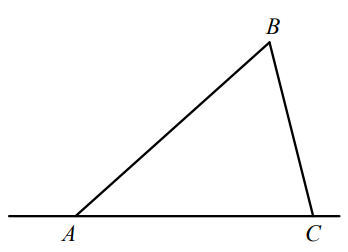
\includegraphics[width=0.30\linewidth]{assets/figure-002.png}
\end{center}
\taskspace

\Needspace{6\baselineskip}
\item Внешние углы треугольника АВС при вершинах А и С равны 154° и 50° соответственно. Определите градусную меру угла АВС.
\begin{center}
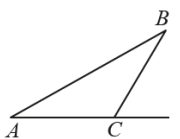
\includegraphics[width=0.30\linewidth]{assets/figure-003.png}
\end{center}
\taskspace

\Needspace{6\baselineskip}
\item Внешние углы треугольника АВС при вершинах А и С равны 160° и 52° соответственно. Определите градусную меру угла АВС.
\begin{center}
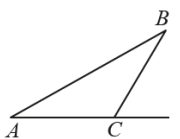
\includegraphics[width=0.30\linewidth]{assets/figure-004.png}
\end{center}
\taskspace

\Needspace{6\baselineskip}
\item Внешние углы треугольника АВС при вершинах А и С равны 80° и 146° соответственно. Определите градусную меру угла АВС.
\begin{center}
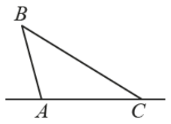
\includegraphics[width=0.30\linewidth]{assets/figure-005.png}
\end{center}
\taskspace

\Needspace{6\baselineskip}
\item Внешние углы треугольника АВС при вершинах А и С равны 78° и 150° соответственно. Определите градусную меру угла АВС.
\begin{center}
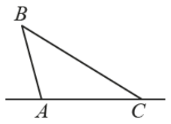
\includegraphics[width=0.30\linewidth]{assets/figure-006.png}
\end{center}
\taskspace

\Needspace{6\baselineskip}
\item Внешние углы треугольника АВС при вершинах А и С равны 160° и 54° соответственно. Определите градусную меру угла АВС.
\begin{center}
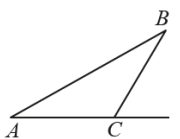
\includegraphics[width=0.30\linewidth]{assets/figure-009.png}
\end{center}
\taskspace

\Needspace{6\baselineskip}
\item Внешние углы треугольника АВС при вершинах А и С равны 74° и 150° соответственно. Определите градусную меру угла АВС.
\begin{center}
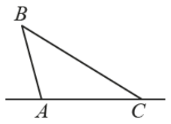
\includegraphics[width=0.30\linewidth]{assets/figure-010.png}
\end{center}
\taskspace

\Needspace{6\baselineskip}
\item Внешние углы треугольника АВС при вершинах А и С равны 70° и 148° соответственно. Определите градусную меру угла АВС.
\begin{center}
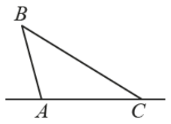
\includegraphics[width=0.30\linewidth]{assets/figure-011.png}
\end{center}
\taskspace

\Needspace{6\baselineskip}
\item Внешние углы треугольника АВС при вершинах А и С равны 156° и 50° соответственно. Определите градусную меру угла АВС.
\begin{center}
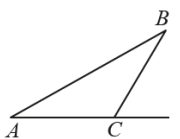
\includegraphics[width=0.30\linewidth]{assets/figure-012.png}
\end{center}
\taskspace

\Needspace{6\baselineskip}
\item Через вершину С треугольника СDЕ параллельно стороне ED провели прямую АВ. По условию СF --- биссектриса угла DСЕ, ∠СDF=40°, ∠СEF=60°. Определите угол АСF. Укажите ответ в градусах.
\begin{center}
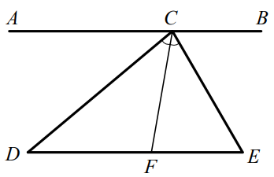
\includegraphics[width=0.30\linewidth]{assets/figure-013.png}
\end{center}
\taskspace

\Needspace{6\baselineskip}
\item В равнобедренном треугольнике АВС с основанием АС проведена биссектриса AD, ∠АDС=132°. Определите угол СВА. Укажите ответ в градусах.
\begin{center}
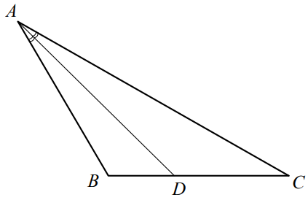
\includegraphics[width=0.30\linewidth]{assets/figure-014.png}
\end{center}
\taskspace

\Needspace{6\baselineskip}
\item Через вершину С треугольника СDЕ параллельно стороне ED провели прямую АВ. По условию СF --- биссектриса угла DСЕ, ∠СDF=42°, ∠СEF=58°. Определите угол АСF. Укажите ответ в градусах.
\begin{center}
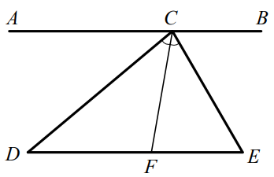
\includegraphics[width=0.30\linewidth]{assets/figure-015.png}
\end{center}
\taskspace

\Needspace{6\baselineskip}
\item В равнобедренном треугольнике АВС с основанием АС проведена биссектриса AD, ∠АDС=150°. Определите угол СВА. Укажите ответ в градусах.
\begin{center}
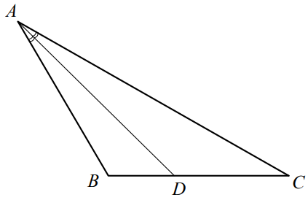
\includegraphics[width=0.30\linewidth]{assets/figure-016.png}
\end{center}
\taskspace

\Needspace{6\baselineskip}
\item Через вершину С треугольника СDЕ параллельно стороне ED провели прямую АВ. По условию СF --- биссектриса угла DСЕ, ∠СDF=54°, ∠СEF=62°. Определите угол АСF. Укажите ответ в градусах.
\begin{center}
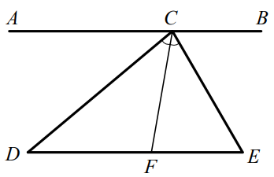
\includegraphics[width=0.30\linewidth]{assets/figure-017.png}
\end{center}
\taskspace

\Needspace{6\baselineskip}
\item В равнобедренном треугольнике АВС с основанием АС проведена биссектриса AD, ∠АDС=126°. Определите угол СВА. Укажите ответ в градусах.
\begin{center}
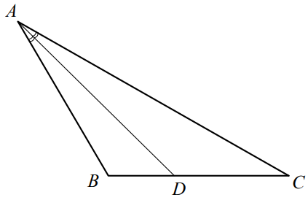
\includegraphics[width=0.30\linewidth]{assets/figure-018.png}
\end{center}
\taskspace

\Needspace{6\baselineskip}
\item Угол B треугольника ABC равен 37°. Внешний угол при вершине A равен 108°. Определите градусную меру внешнего угла при вершине C.

\taskspace

\Needspace{6\baselineskip}
\item Угол B треугольника ABC равен 51°. Внешний угол при вершине A равен 124°. Определите градусную меру внешнего угла при вершине C.

\taskspace

\Needspace{6\baselineskip}
\item Угол B треугольника ABC равен 75°. Внешний угол при вершине A равен 130°. Определите градусную меру внешнего угла при вершине C.

\taskspace

\Needspace{6\baselineskip}
\item Угол B треугольника ABC равен 48°. Внешний угол при вершине A равен 112°. Определите градусную меру внешнего угла при вершине C.

\taskspace

\Needspace{6\baselineskip}
\item В равнобедренном треугольнике ABC с основанием AC проведена биссектриса AD, ∠ADB = 102° (D лежит на боковой стороне BC). Определите угол BAC.

\taskspace

\Needspace{6\baselineskip}
\item В равнобедренном треугольнике ABC (AB = BC) проведена биссектриса AD угла A, причём D лежит на стороне BC. По условию ∠ADC = 117°. Определите угол B.

\taskspace

\Needspace{6\baselineskip}
\item В равнобедренном треугольнике ABC с основанием AC проведена биссектриса BK (K на AC). Точка D на продолжении стороны AB за вершину B такова, что BD = BC. Угол ADC = 55°. Определите угол ABC.

\taskspace

\Needspace{6\baselineskip}
\item В равнобедренном треугольнике ABC (AC --- основание) проведена биссектриса AM угла A, M лежит на BC. Определите угол ABC, если ∠AMC = 124°.

\taskspace

\Needspace{6\baselineskip}
\item В равнобедренном треугольнике ABC с основанием BC проведена биссектриса AD угла A, D лежит на BC. Определите угол BAC, если ∠ADC = 112°.

\taskspace

\Needspace{6\baselineskip}
\item В равнобедренном треугольнике ABC (AB = BC) проведена биссектриса CD угла C, D лежит на AB. Определите угол ABC, если ∠CDA = 99°.

\taskspace

\Needspace{6\baselineskip}
\item В равнобедренном треугольнике ABC с основанием AC проведена биссектриса BF (F на AC). Точка D на стороне AB такова, что FD ∥ BC. Определите угол ABC, если ∠BDF = 108°.

\taskspace

\Needspace{6\baselineskip}
\item В равнобедренном треугольнике ABC (AB = BC) проведена биссектриса AK угла A, K на BC. Определите угол ABC, если ∠AKC = 138°.

\taskspace

\Needspace{6\baselineskip}
\item В равнобедренном треугольнике ABC с основанием AC проведена биссектриса AM угла A (M на BC). Определите угол AMB, если ∠ACB = 42°.

\taskspace

\Needspace{6\baselineskip}
\item В равнобедренном треугольнике ABC (AC --- основание) проведена биссектриса BD (D на AC). На стороне BC отмечена точка E такая, что DE ∥ AB. Определите угол ABC, если ∠CDE = 144°.

\taskspace

\Needspace{6\baselineskip}
\item В равнобедренном треугольнике ABC с основанием AC проведена биссектриса AD (D лежит на стороне BC). По условию угол ADB = 132°. Определите угол CBA. Укажите ответ в градусах.

\taskspace

\end{enumerate}

\newpage

\section*{Блок II. Задание МЦКО 2}

\blocknote{Анализ геометрических высказываний.}

\begin{enumerate}[resume]

\Needspace{6\baselineskip}
\item Отметьте все утверждения, которые являются верными.
\begin{enumerate}[label=\arabic*),leftmargin=8mm,itemsep=0.25em,topsep=0.35em]
\item Существует равнобедренный треугольник, в котором один из углов в 2 раза больше другого.
\item В любом прямоугольном треугольнике один из катетов в 2 раза меньше другого.
\item При пересечении двух любых прямых сумма пары образованных ими вертикальных углов равна 180°.
\item В любом треугольнике длина одной стороны меньше суммы длин двух других сторон.
\end{enumerate}

\taskspace

\Needspace{6\baselineskip}
\item Отметьте все утверждения, которые являются верными.
\begin{enumerate}[label=\arabic*),leftmargin=8mm,itemsep=0.25em,topsep=0.35em]
\item Смежные углы всегда равны.
\item Тупоугольный треугольник может быть равнобедренным.
\item Если один из внешних углов треугольника острый, то внешние углы при других вершинах треугольника тупые.
\item Если две стороны одного прямоугольного треугольника равны двум сторонам другого прямоугольного треугольника, то эти треугольники всегда равны.
\end{enumerate}

\taskspace

\Needspace{6\baselineskip}
\item Отметьте все утверждения, которые являются верными.
\begin{enumerate}[label=\arabic*),leftmargin=8mm,itemsep=0.25em,topsep=0.35em]
\item Любые два угла, сумма которых равна 180°, являются смежными.
\item В прямоугольном треугольнике с углом 60° гипотенуза в два раза больше одного из катетов.
\item Внешний угол треугольника больше любого внутреннего угла этого треугольника.
\item Если в треугольнике есть два равных угла, то в этом треугольнике всегда есть две равные стороны.
\end{enumerate}

\taskspace

\Needspace{6\baselineskip}
\item Отметьте все утверждения, которые являются верными.
\begin{enumerate}[label=\arabic*),leftmargin=8mm,itemsep=0.25em,topsep=0.35em]
\item Сумма смежных углов равна 90°.
\item В прямоугольном треугольнике любой внешний угол больше 85°.
\item Если три стороны одного треугольника равны трём сторонам другого треугольника, то эти треугольники равны.
\item Треугольник, в котором высота совпадает с его биссектрисой и медианой, является равносторонним.
\end{enumerate}

\taskspace

\Needspace{6\baselineskip}
\item Отметьте все утверждения, которые являются верными.
\begin{enumerate}[label=\arabic*),leftmargin=8mm,itemsep=0.25em,topsep=0.35em]
\item В прямоугольном треугольнике любой внешний угол больше 88°.
\item Если прямая a параллельна двум различным прямым b и c, то прямые b и c всегда перпендикулярны.
\item Треугольник, в котором высота является его биссектрисой, является равнобедренным.
\item Если сторона и два угла одного треугольника равны стороне и двум углам другого треугольника, то эти треугольники всегда равны.
\end{enumerate}

\taskspace

\Needspace{6\baselineskip}
\item Отметьте все утверждения, которые являются верными.
\begin{enumerate}[label=\arabic*),leftmargin=8mm,itemsep=0.25em,topsep=0.35em]
\item Сумма смежных углов равна 180°.
\item Если в треугольнике есть тупой угол, то треугольник не может быть равнобедренным.
\item Внешний угол треугольника равен сумме внутренних углов этого треугольника.
\item Если гипотенуза и острый угол одного прямоугольного треугольника равны гипотенузе и углу другого прямоугольного треугольника, то эти треугольники равны.
\end{enumerate}

\taskspace

\Needspace{6\baselineskip}
\item Отметьте все утверждения, которые являются верными.
\begin{enumerate}[label=\arabic*),leftmargin=8mm,itemsep=0.25em,topsep=0.35em]
\item Если прямая пересекает одну из перпендикулярных прямых, то она параллельна другой.
\item Треугольник, в котором два угла равны, является равнобедренным.
\item Если катет и острый угол одного прямоугольного треугольника равны катету и углу другого прямоугольного треугольника, то эти треугольники всегда равны.
\item Внешний угол треугольника больше любого внутреннего угла треугольника, не смежного с ним.
\end{enumerate}

\taskspace

\Needspace{6\baselineskip}
\item Отметьте все утверждения, которые являются верными.
\begin{enumerate}[label=\arabic*),leftmargin=8mm,itemsep=0.25em,topsep=0.35em]
\item Вертикальные углы всегда равны.
\item В любом прямоугольном треугольнике один из катетов в два раза меньше гипотенузы.
\item Существует равнобедренный треугольник, в котором один из углов в 4 раза больше другого.
\item Если две стороны и угол одного треугольника равны двум сторонам и углу другого треугольника, то эти треугольники всегда равны.
\end{enumerate}

\taskspace

\Needspace{6\baselineskip}
\item Отметьте все утверждения, которые являются верными.
\begin{enumerate}[label=\arabic*),leftmargin=8mm,itemsep=0.25em,topsep=0.35em]
\item Сумма острых углов прямоугольного треугольника равна 90°.
\item На прямой от данной точки можно отложить только один отрезок данной длины.
\item Если углы одного треугольника соответственно равны углам другого треугольника, то эти треугольники всегда равны.
\item Существует равнобедренный треугольник, в котором один из углов в 5 раз больше другого.
\end{enumerate}

\taskspace

\Needspace{6\baselineskip}
\item Отметьте все утверждения, которые являются верными.
\begin{enumerate}[label=\arabic*),leftmargin=8mm,itemsep=0.25em,topsep=0.35em]
\item Если в треугольнике ABC углы A и B равны соответственно 40° и 70°, то внешний угол этого треугольника при вершине C равен 70°.
\item Центром окружности, описанной около любого треугольника, является точка пересечения биссектрис этого треугольника.
\item Каждая из биссектрис равнобедренного треугольника является его высотой.
\item Через любые две различные точки плоскости можно провести не более одной прямой.
\end{enumerate}

\taskspace

\Needspace{6\baselineskip}
\item Отметьте все утверждения, которые являются верными.
\begin{enumerate}[label=\arabic*),leftmargin=8mm,itemsep=0.25em,topsep=0.35em]
\item Касательная к окружности параллельна радиусу, проведённому в точку касания.
\item В любом треугольнике биссектриса делит пополам сторону, которую она пересекает.
\item Две различные прямые, перпендикулярные третьей прямой, параллельны друг другу.
\item Если угол острый, то смежный с ним угол также является острым.
\end{enumerate}

\taskspace

\Needspace{6\baselineskip}
\item Отметьте все утверждения, которые являются верными.
\begin{enumerate}[label=\arabic*),leftmargin=8mm,itemsep=0.25em,topsep=0.35em]
\item Через любые три различные точки плоскости можно провести не менее одной окружности.
\item Треугольник со сторонами 2, 4, 7 существует.
\item Существует треугольник, внешний угол которого равен сумме двух любых внутренних углов этого треугольника.
\item Две прямые, каждая из которых перпендикулярна третьей прямой, перпендикулярны.
\end{enumerate}

\taskspace

\Needspace{6\baselineskip}
\item Отметьте все утверждения, которые являются верными.
\begin{enumerate}[label=\arabic*),leftmargin=8mm,itemsep=0.25em,topsep=0.35em]
\item Сумма углов треугольника равна 360°.
\item Центром окружности, описанной около правильного треугольника, является точка пересечения его высот.
\item Если две прямые перпендикулярны третьей, то эти две прямые параллельны.
\item Внешний угол треугольника всегда больше смежного ему внутреннего угла.
\end{enumerate}

\taskspace

\Needspace{6\baselineskip}
\item Отметьте все утверждения, которые являются верными.
\begin{enumerate}[label=\arabic*),leftmargin=8mm,itemsep=0.25em,topsep=0.35em]
\item Если две стороны и угол между ними одного треугольника соответственно равны двум сторонам и углу между ними другого треугольника, то такие треугольники равны.
\item Через любую точку, лежащую вне окружности, можно провести только одну касательную к этой окружности.
\item Если при пересечении двух данных прямых третьей внутренние накрест лежащие углы равны, то данные прямые параллельны.
\item Если в треугольнике ABC углы A и B равны соответственно 40° и 70°, то внешний угол этого треугольника при вершине C равен 110°
\end{enumerate}

\taskspace

\Needspace{6\baselineskip}
\item Отметьте все утверждения, которые являются верными.
\begin{enumerate}[label=\arabic*),leftmargin=8mm,itemsep=0.25em,topsep=0.35em]
\item Смежные углы равны.
\item В любом тупоугольном треугольнике есть острый угол.
\item Через точку, не лежащую на данной прямой, можно провести прямую, параллельную данной.
\item Каждая биссектриса равнобедренного треугольника является его высотой.
\end{enumerate}

\taskspace

\Needspace{6\baselineskip}
\item Отметьте все утверждения, которые являются верными.
\begin{enumerate}[label=\arabic*),leftmargin=8mm,itemsep=0.25em,topsep=0.35em]
\item Любая точка, лежащая на биссектрисе угла, равноудалена от сторон этого угла.
\item Если в треугольнике есть один острый угол, то этот треугольник остроугольный.
\item В прямоугольном треугольнике квадрат гипотенузы равен разности квадратов катетов.
\item В любом треугольнике хотя бы один из углов не превосходит 60°.
\end{enumerate}

\taskspace

\Needspace{6\baselineskip}
\item Отметьте все утверждения, которые являются верными.
\begin{enumerate}[label=\arabic*),leftmargin=8mm,itemsep=0.25em,topsep=0.35em]
\item Сумма углов выпуклого четырёхугольника равна 360 градусам.
\item В прямоугольном треугольнике гипотенуза равна сумме катетов.
\item Площадь прямоугольника равна произведению длин его смежных сторон.
\item Если три угла одного треугольника равны соответственно трём углам другого треугольника, то такие треугольники равны.
\end{enumerate}

\taskspace

\Needspace{6\baselineskip}
\item Отметьте все утверждения, которые являются верными.
\begin{enumerate}[label=\arabic*),leftmargin=8mm,itemsep=0.25em,topsep=0.35em]
\item Против большей стороны треугольника лежит меньший угол.
\item Существует квадрат, который нельзя вписать в окружность
\item Площадь трапеции равна произведению средней линии на высоту.
\item Через любые четыре точки, не принадлежащие одной прямой, проходит единственная окружность.
\end{enumerate}

\taskspace

\Needspace{6\baselineskip}
\item Отметьте все утверждения, которые являются верными.
\begin{enumerate}[label=\arabic*),leftmargin=8mm,itemsep=0.25em,topsep=0.35em]
\item Через точку, не лежащую на данной прямой, можно провести прямую, перпендикулярную этой прямой.
\item Треугольник со сторонами 1, 2, 4 существует.
\item Сумма квадратов диагоналей прямоугольника равна сумме кубов всех его сторон.
\item Если расстояние от точки до прямой меньше 1, то и длина любой наклонной, проведенной из данной точки к прямой, меньше 1.
\end{enumerate}

\taskspace

\Needspace{6\baselineskip}
\item Отметьте все утверждения, которые являются верными.
\begin{enumerate}[label=\arabic*),leftmargin=8mm,itemsep=0.25em,topsep=0.35em]
\item Две окружности пересекаются, если радиус одной окружности больше радиуса другой окружности.
\item Если при пересечении двух прямых третьей прямой внутренние накрест лежащие углы равны, то эти прямые параллельны.
\item У равнобедренного треугольника есть центр симметрии.
\item Около любого правильного многоугольника можно описать более одной окружности.
\end{enumerate}

\taskspace

\Needspace{6\baselineskip}
\item Отметьте все утверждения, которые являются верными.
\begin{enumerate}[label=\arabic*),leftmargin=8mm,itemsep=0.25em,topsep=0.35em]
\item Через любые три точки проходит ровно одна прямая.
\item Сумма смежных углов равна 900.
\item Если при пересечении двух прямых третьей прямой соответственные углы составляют в сумме то эти две прямые параллельны.
\item Через любые две точки проходит не более одной прямой.
\end{enumerate}

\taskspace

\Needspace{6\baselineskip}
\item Отметьте все утверждения, которые являются верными.
\begin{enumerate}[label=\arabic*),leftmargin=8mm,itemsep=0.25em,topsep=0.35em]
\item Если две стороны треугольника равны 3 и 5, то его третья сторона больше 3.
\item Внешний угол треугольника равен сумме двух его внутренних углов.
\item Если две стороны и угол одного треугольника соответственно равны двум сторонам и углу другого треугольника, то такие треугольники равны.
\item Если две стороны треугольника равны 3 и 4, то его третья сторона меньше 7.
\end{enumerate}

\taskspace

\Needspace{6\baselineskip}
\item Отметьте все утверждения, которые являются верными.
\begin{enumerate}[label=\arabic*),leftmargin=8mm,itemsep=0.25em,topsep=0.35em]
\item В треугольнике против меньшего угла лежит большая сторона.
\item Если один угол треугольника больше 120°, то два других его угла меньше 30°.
\item Если все стороны треугольника меньше 1, то и хотя бы одна его высота больше 1.
\item Сумма острых углов прямоугольного треугольника не превосходит 90°.
\end{enumerate}

\taskspace

\Needspace{6\baselineskip}
\item Отметьте все утверждения, которые являются верными.
\begin{enumerate}[label=\arabic*),leftmargin=8mm,itemsep=0.25em,topsep=0.35em]
\item Сумма смежных углов всегда равна 180°.
\item Если в треугольнике есть тупой угол, то треугольник не может быть равнобедренным.
\item Внешний угол треугольника равен сумме двух внутренних углов, не смежных с ним.
\item Если гипотенуза и острый угол одного прямоугольного треугольника равны гипотенузе и острому углу другого, то эти треугольники равны.
\end{enumerate}

\taskspace

\Needspace{6\baselineskip}
\item Отметьте все утверждения, которые являются верными.
\begin{enumerate}[label=\arabic*),leftmargin=8mm,itemsep=0.25em,topsep=0.35em]
\item Если прямая пересекает одну из двух перпендикулярных прямых, то она параллельна другой.
\item В треугольнике против большей стороны лежит больший угол.
\item Если катет и прилежащий острый угол одного прямоугольного треугольника равны катету и прилежащему острому углу другого, то треугольники равны.
\item Внешний угол треугольника всегда больше любого внутреннего угла.
\end{enumerate}

\taskspace

\Needspace{6\baselineskip}
\item Отметьте все утверждения, которые являются верными.
\begin{enumerate}[label=\arabic*),leftmargin=8mm,itemsep=0.25em,topsep=0.35em]
\item Вертикальные углы равны.
\item В любом прямоугольном треугольнике катет, лежащий против угла 30°, равен половине гипотенузы.
\item Если два угла одного треугольника равны двум углам другого, то такие треугольники всегда равны.
\item Существует равнобедренный треугольник, в котором один угол в 4 раза больше другого.
\end{enumerate}

\taskspace

\Needspace{6\baselineskip}
\item Отметьте все утверждения, которые являются верными.
\begin{enumerate}[label=\arabic*),leftmargin=8mm,itemsep=0.25em,topsep=0.35em]
\item Сумма острых углов прямоугольного треугольника равна 90°.
\item На прямой от данной точки можно отложить ровно один отрезок заданной длины.
\item Если три угла одного треугольника равны трём углам другого, то треугольники равны.
\item В равнобедренном треугольнике биссектриса, проведённая к основанию, является медианой и высотой.
\end{enumerate}

\taskspace

\Needspace{6\baselineskip}
\item Отметьте все утверждения, которые являются верными.
\begin{enumerate}[label=\arabic*),leftmargin=8mm,itemsep=0.25em,topsep=0.35em]
\item Если две стороны и угол между ними одного треугольника равны двум сторонам и углу между ними другого, то треугольники равны.
\item В тупоугольном треугольнике все углы тупые.
\item Через точку, не лежащую на прямой, можно провести только одну прямую, параллельную данной.
\item Любой равносторонний треугольник является равнобедренным.
\end{enumerate}

\taskspace

\Needspace{6\baselineskip}
\item Отметьте все утверждения, которые являются верными.
\begin{enumerate}[label=\arabic*),leftmargin=8mm,itemsep=0.25em,topsep=0.35em]
\item Если в треугольнике два угла равны, то он равнобедренный.
\item Внешний угол треугольника может быть меньше смежного с ним внутреннего угла.
\item Если катет и гипотенуза одного прямоугольного треугольника равны катету и гипотенузе другого, то треугольники равны.
\item Сумма вертикальных углов всегда равна 180°.
\end{enumerate}

\taskspace

\Needspace{6\baselineskip}
\item Отметьте все утверждения, которые являются верными.
\begin{enumerate}[label=\arabic*),leftmargin=8mm,itemsep=0.25em,topsep=0.35em]
\item Если прямая параллельна одной из двух параллельных прямых, то она параллельна и другой.
\item В любом треугольнике хотя бы два угла острые.
\item Если сторона и два прилежащих к ней угла одного треугольника равны стороне и двум прилежащим углам другого, то треугольники равны.
\item В равнобедренном треугольнике углы при основании всегда острые.
\end{enumerate}

\taskspace

\end{enumerate}

\newpage

\section*{Блок III. Задание МЦКО 3}

\blocknote{Треугольники и параллельные прямые.}

\begin{enumerate}[resume]

\Needspace{6\baselineskip}
\item В треугольнике ABC проведены медиана BM и высота BH. По условию AH = 54, BC = BM. Вычислите длину стороны AC.

\taskspace

\Needspace{6\baselineskip}
\item В треугольнике АВС угол АВС равен 120°, AB = ВС, ВМ --- медиана. На луче ВМ отметили точку F такую, что угол ВАF = 90°. Определите АВ, если FM = 63.

\taskspace

\Needspace{6\baselineskip}
\item В треугольнике АВС угол С равен 56°, а угол между прямыми, содержащими биссектрису угла ВАС и биссектрису внешнего угла С, равен 54°. Определите градусную меру угла АВС.

\taskspace

\Needspace{6\baselineskip}
\item В треугольнике АВС угол АВС равен 120°, AB = BC, ВМ --- медиана. На луче ВМ отметили точку F такую, что угол ВАF = 90°. Определите АВ, если FM = 27.

\taskspace

\Needspace{6\baselineskip}
\item В треугольнике АВС угол АВС равен 120°, АB = BC, BM --- медиана. На луче ВМ отметили точку F такую, что угол ВАF = 90°. Определите ВF, если FM = 36.

\taskspace

\Needspace{6\baselineskip}
\item В треугольнике АВС угол АВС равен 120°, AB = BC, ВМ --- медиана. На луче ВМ отметили точку F такую, что угол ВАF = 90°. Определите АВ, если FM = 81.

\taskspace

\Needspace{6\baselineskip}
\item В треугольнике ABC угол B равен 120°, внешний угол при вершине C равен 150°, сторона BC равна 44. Из вершины A проведена высота AH. Вычислите длину отрезка BH.

\taskspace

\Needspace{6\baselineskip}
\item В треугольнике АВС угол АВС равен 120°, AB = BC, ВМ --- медиана. На луче ВМ отметили точку F такую, что BAF = 90°. Определите ВF, если FM = 18.

\taskspace

\Needspace{6\baselineskip}
\item В треугольнике ABC угол B равен 120°, внешний угол при вершине C равен 150°, сторона BC равна 12. Из вершины A проведена высота AH. Вычислите длину отрезка BH.

\taskspace

\Needspace{6\baselineskip}
\item В равнобедренном треугольнике ABC с основанием AC проведена биссектриса AM. Угол AMC равен 78° . Определите угол при основании этого треугольника.

\taskspace

\Needspace{6\baselineskip}
\item В треугольнике ABC угол B равен 120°, внешний угол при вершине C равен 150°, сторона BC равна 50. Из вершины A проведена высота AH. Вычислите длину отрезка BH.

\taskspace

\Needspace{6\baselineskip}
\item В равнобедренном треугольнике ABC с основанием AC проведена биссектриса AM. Угол AMB равен 69°. Определите угол при основании этого треугольника.

\taskspace

\Needspace{6\baselineskip}
\item В треугольнике ABC угол B равен 120°, внешний угол при вершине C равен 150°, сторона BC равна 38. Из вершины A проведена высота AH. Вычислите длину отрезка BH.

\taskspace

\Needspace{6\baselineskip}
\item В равнобедренном треугольнике ABC с основанием AC проведена биссектриса AM. Угол AMC равен 78° . Определите угол при основании этого треугольника.

\taskspace

\Needspace{6\baselineskip}
\item В треугольнике ABC угол B равен 120°, внешний угол при вершине C равен 150°, сторона BC равна 34. Из вершины A проведена высота AH. Вычислите длину отрезка BH.

\taskspace

\Needspace{6\baselineskip}
\item В равнобедренном треугольнике ABC с основанием AC проведена биссектриса AM. Угол AMB равен 69°. Определите угол при основании этого треугольника.

\taskspace

\Needspace{6\baselineskip}
\item В треугольнике ABC угол B равен 120°, внешний угол при вершине C равен 150°, сторона BC равна 8. Из вершины A проведена высота AH. Вычислите длину отрезка BH.

\taskspace

\Needspace{6\baselineskip}
\item В прямоугольном треугольнике АВС угол B прямой, BC=5, AC=10. Биссектрисы углов АВС и АСВ пересекаются в точке О. Вычислите величину угла ВОС. Укажите ответ в градусах.

\taskspace

\Needspace{6\baselineskip}
\item На продолжении стороны AC равнобедренного треугольника ABC с основанием BC отметили точку D так, что CD = BC и точка C находится между точками A и D. Вычислите величину угла CDB если угол BAC равен 72°. Укажите ответ в градусах.

\taskspace

\Needspace{6\baselineskip}
\item В треугольнике АВС угол АСВ равен 48°, угол CAD равен 22°, AD --- биссектриса. Определите величину угла АВС. Укажите ответ в градусах.

\taskspace

\Needspace{6\baselineskip}
\item Сторона BC треугольника ABC продолжена за точку B. На продолжении отмечена точка D так, что AB = DB. Вычислите величину угла BAD, если угол ACB равен 70°, а угол BAC равен 34°. Ответ дайте в градусах.

\taskspace

\Needspace{6\baselineskip}
\item В треугольнике АВС угол АСВ равен 37°, угол CAD равен 28°, AD --- биссектриса. Определите величину угла АВС. Укажите ответ в градусах.

\taskspace

\Needspace{6\baselineskip}
\item Сторона BC треугольника ABC продолжена за точку B. На продолжении отмечена точка D так, что AB = DB. Вычислите величину угла BAD, если угол ACB равен 80°, а угол BAC равен 28°. Ответ дайте в градусах.

\taskspace

\Needspace{6\baselineskip}
\item В треугольнике АВС угол АСВ равен 47°, угол CAD равен 23°, AD --- биссектриса. Определите величину угла АВС. Укажите ответ в градусах.

\taskspace

\Needspace{6\baselineskip}
\item Сторона BC треугольника ABC продолжена за точку C. На продолжении отмечена точка D так, что AC = CD. Вычислите величину угла DAC, если угол ABC равен 85°, а угол BAC равен 45°. Ответ дайте в градусах.

\taskspace

\Needspace{6\baselineskip}
\item В треугольнике АВС угол АСВ равен 53°, угол CAD равен 24°, AD --- биссектриса. Определите величину угла АВС. Укажите ответ в градусах.

\taskspace

\Needspace{6\baselineskip}
\item Сторона BC треугольника ABC продолжена за точку C. На продолжении отмечена точка D так, что AC = CD. Вычислите величину угла DAC, если угол ABC равен 78°, а угол BAC равен 20°. Ответ дайте в градусах.

\taskspace

\Needspace{6\baselineskip}
\item Биссектриса внешнего угла при вершине В треугольника ABC параллельна стороне АС. Определите величину угла САВ, если ∠ABC = 36°. Укажите ответ в градусах. Запишите решение и ответ.

\taskspace

\Needspace{6\baselineskip}
\item Биссектриса внешнего угла при вершине В треугольника ABC параллельна стороне АС. Определите величину угла САВ, если ∠ABC = 32°. Укажите ответ в градусах.

\taskspace

\Needspace{6\baselineskip}
\item Биссектриса внешнего угла при вершине В треугольника ABC параллельна стороне АС. Определите величину угла САВ, если ∠ABC = 30°. Укажите ответ в градусах.

\taskspace

\end{enumerate}

\newpage

\section*{Блок IV. Задание МЦКО 4}

\blocknote{Геометрические задачи повышенного уровня.}

\begin{enumerate}[resume]

\Needspace{6\baselineskip}
\item Рассмотрим треугольники ABC и ADC, причём точки B и D лежат по разные стороны от прямой AC. Углы ABC и ADC равны 77° и 74° соответственно. Определите градусную меру угла BAD, если AB = AC = AD.

\taskspace

\Needspace{6\baselineskip}
\item В треугольнике АВС угол С равен 28°, а угол между прямыми, содержащими биссектрису угла АВС и биссектрису внешнего угла С, равен 52°. Определите градусную меру угла ВАС.

\taskspace

\Needspace{6\baselineskip}
\item В треугольнике АВС угол С равен 32°, а угол между прямыми, содержащими биссектрису угла АВС и биссектрису внешнего угла С, равен 18°. Определите градусную меру угла ВАС.

\taskspace

\Needspace{6\baselineskip}
\item В треугольнике АВС угол С равен 52°, а угол между прямыми, содержащими биссектрису угла АВС и биссектрису внешнего угла С, равен 48°. Определите градусную меру угла ВАС.

\taskspace

\Needspace{6\baselineskip}
\item В треугольнике АВС угол С равен 56°, а угол между прямыми, содержащими биссектрису угла ВАС и биссектрису внешнего угла С, равен 54°.Определите градусную меру угла АВС.

\taskspace

\Needspace{6\baselineskip}
\item B треугольнике АВС угол С равен 26°, а угол между прямыми, содержащими биссектрису угла BAC и биссектрису внешнего угла C, равен 14°. Определите градусную меру угла АВС.

\taskspace

\Needspace{6\baselineskip}
\item B треугольнике АВС угол С равен 24°, а угол между прямыми, содержащими биссектрису угла BAC и биссектрису внешнего угла С, равен 56°. Определите градусную меру угла АВС.

\taskspace

\Needspace{6\baselineskip}
\item В треугольнике АВС угол С равен 38°, а угол между прямыми, содержащими биссектрису угла ВАС и биссектрису внешнего угла С, равен 42°. Определите градусную меру угла АВС.

\taskspace

\Needspace{6\baselineskip}
\item B треугольнике АВС угол С равен 44°, а угол между прямыми, содержащими биссектрису угла АВС и биссектрису внешнего угла С, равен 26°. Определите градусную меру угла ВАС.

\taskspace

\Needspace{6\baselineskip}
\item В равнобедренном треугольнике АВС с основанием ВС проведена медиана АМ. Определите медиану АМ, если периметр треугольника АВС равен 56 см, а периметр треугольника АВМ равен 42 см.

\taskspace

\Needspace{6\baselineskip}
\item В треугольнике ABC проведены медиана BM и высота BH. По условию AC = 84 и BC = BM. Определите AH.

\taskspace

\Needspace{6\baselineskip}
\item В треугольнике ABC BM --- медиана и BH --- высота. По условию AC = 216, HC = 54 и ∠ACB = 40°. Определите угол AMB. Укажите ответ в градусах.

\taskspace

\Needspace{6\baselineskip}
\item Рассмотрим треугольники ABC и ADC, причём точки B и D лежат по разные стороны от прямой AC. Углы ABC и ADC равны 77° и 74° соответственно. Определите градусную меру угла BAD, если AB = AC = AD.

\taskspace

\Needspace{6\baselineskip}
\item Рассмотрим треугольники ABC и ADC, причём точки B и D лежат по разные стороны от прямой AC. Углы ABC и ADC равны 80° и 70° соответственно. Определите градусную меру угла BAD, если AB = AC = AD.

\taskspace

\Needspace{6\baselineskip}
\item Рассмотрим треугольники ABC и ADC, причём точки B и D лежат по разные стороны от прямой AC. Углы ABC и ADC равны 65° и 55° соответственно. Определите градусную меру угла BAD, если AB = AC = AD.

\taskspace

\Needspace{6\baselineskip}
\item Рассмотрим треугольники ABC и ADC, причём точки B и D лежат по разные стороны от прямой AC. Углы ABC и ADC равны 50° и 40° соответственно. Определите градусную меру угла BAD, если AB = AC = AD.

\taskspace

\Needspace{6\baselineskip}
\item Рассмотрим треугольники ABC и ADC, причём точки B и D лежат по разные стороны от прямой AC. Углы ABC и ADC равны 85° и 75° соответственно. Определите градусную меру угла BAD, если AB = AC = AD.

\taskspace

\Needspace{6\baselineskip}
\item Рассмотрим треугольники ABC и ADC, причём точки B и D лежат по разные стороны от прямой AC. Углы ABC и ADC равны 30° и 20° соответственно. Определите градусную меру угла BAD, если AB = AC = AD.

\taskspace

\Needspace{6\baselineskip}
\item Рассмотрим треугольники ABC и ADC, причём точки B и D лежат по разные стороны от прямой AC. Углы ABC и ADC равны 44° и 38° соответственно. Определите градусную меру угла BAD, если AB = AC = AD.

\taskspace

\Needspace{6\baselineskip}
\item Рассмотрим треугольники ABC и ADC, причём точки B и D лежат по разные стороны от прямой AC. Углы ABC и ADC равны 72° и 68° соответственно. Определите градусную меру угла BAD, если AB = AC = AD.

\taskspace

\Needspace{6\baselineskip}
\item В окружности с центром O проведены диаметры AC и BD. Определите величину угла BOA в градусах, если угол DBC равен 48°.

\taskspace

\Needspace{6\baselineskip}
\item В окружности с центром O проведены диаметры AC и BD. Определите величину угла BOA в градусах, если угол DBC равен 55°.

\taskspace

\Needspace{6\baselineskip}
\item В окружности с центром O проведены диаметры AC и BD. Определите величину угла BOA в градусах, если угол DBC равен 51°.

\taskspace

\Needspace{6\baselineskip}
\item В окружности с центром O проведены диаметры AC и BD. Определите градусную меру угла BOA, если угол DBC равен 30°.

\taskspace

\Needspace{6\baselineskip}
\item В окружности с центром O проведены диаметры AC и BD. Определите градусную меру угла BOA, если угол DBC равен 25°.

\taskspace

\Needspace{6\baselineskip}
\item В окружности с центром O проведены диаметры AC и BD. Определите величину угла AOD в градусах, если угол ACB равен 55°.

\taskspace

\Needspace{6\baselineskip}
\item В окружности с центром O проведены диаметры AC и BD. Определите величину угла AOD в градусах, если угол ACB равен 56°.

\taskspace

\Needspace{6\baselineskip}
\item В окружности с центром O проведены диаметры AC и BD. Определите градусную меру угла AOD, если угол ACB равен 32°.

\taskspace

\Needspace{6\baselineskip}
\item В окружности с центром O проведены диаметры AC и BD. Определите градусную меру угла AOD, если угол ACB равен 18°.

\taskspace

\Needspace{6\baselineskip}
\item В окружности с центром O проведены диаметры AC и BD. Определите градусную меру угла AOD, если угол ACB равен 71°.

\taskspace

\end{enumerate}

\newpage

\section*{Блок V. Задание МЦКО 5}

\blocknote{Вероятность и статистика: логика.}

\begin{enumerate}[resume]

\Needspace{6\baselineskip}
\item Катя младше Тани, но старше Даши. Ксюша не младше Даши. Отметьте все утверждения, которые являются верными.
\begin{enumerate}[label=\arabic*),leftmargin=8mm,itemsep=0.25em,topsep=0.35em]
\item Таня и Даша одного возраста.
\item Среди указанных девочек нет никого младше Даши.
\item Таня старше Даши.
\item Таня и Катя одного возраста.
\end{enumerate}

\taskspace

\Needspace{6\baselineskip}
\item Олег на 3 см выше Пети и на 5 см выше Толи. Коля на 4 см выше Пети. Отметьте все утверждения, которые являются верными.
\begin{enumerate}[label=\arabic*),leftmargin=8mm,itemsep=0.25em,topsep=0.35em]
\item Олег - самый высокий среди указанных мальчиков.
\item Коля выше Толи на 6 см.
\item Олег ниже Коли.
\item Петя выше Толи на 1 см.
\end{enumerate}

\taskspace

\Needspace{6\baselineskip}
\item Витя на 3 см ниже Бори и на 6 см ниже Егора. Боря на 4 см выше Димы. Отметьте все утверждения, которые являются верными.
\begin{enumerate}[label=\arabic*),leftmargin=8mm,itemsep=0.25em,topsep=0.35em]
\item Дима выше Вити.
\item Егор выше Бори на 2 см.
\item Дима ниже Егора на 7 см.
\item Среди указанных мальчиков нет двоих одного роста.
\end{enumerate}

\taskspace

\Needspace{6\baselineskip}
\item У Лены на 10 наклеек больше, чем у Юли, и на 15 больше, чем у Оли. У Юли на 5 наклеек меньше, чем у Иры. Отметьте все утверждения, которые являются верными.
\begin{enumerate}[label=\arabic*),leftmargin=8mm,itemsep=0.25em,topsep=0.35em]
\item У Юли больше наклеек, чем у Оли.
\item Среди указанных девочек больше всего наклеек у Иры.
\item У Лены на 5 наклеек больше, чем у Иры.
\item У Оли на 5 наклеек меньше, чем у Иры.
\end{enumerate}

\taskspace

\Needspace{6\baselineskip}
\item У Маши на 5 наклеек больше, чем у Яны, и на 15 больше, чем у Риты. У Яны на 10 наклеек меньше, чем у Ани. Отметьте все утверждения, которые являются верными.
\begin{enumerate}[label=\arabic*),leftmargin=8mm,itemsep=0.25em,topsep=0.35em]
\item У Ани на 20 наклеек больше, чем у Риты.
\item Среди указанных девочек больше всего наклеек у Маши.
\item У Яны на 5 наклеек больше, чем у Риты.
\item У Риты наклеек меньше, чем у Яны.
\end{enumerate}

\taskspace

\Needspace{6\baselineskip}
\item Егор на 8 см выше Димы и на 5 см выше Вити. Дима на 4 см ниже Бори. Отметьте все утверждения, которые являются верными.
\begin{enumerate}[label=\arabic*),leftmargin=8mm,itemsep=0.25em,topsep=0.35em]
\item Витя выше Димы на 3 см.
\item Боря ниже Вити.
\item Егор выше Бори на 3 см.
\item Среди указанных мальчиков наименьший рост у Димы.
\end{enumerate}

\taskspace

\Needspace{6\baselineskip}
\item У Маши на 15 наклеек меньше, чем у Риты, и на 10 меньше, чем у Ани. У Ани на 15 наклеек больше, чем у Яны. Отметьте все утверждения, которые являются верными.
\begin{enumerate}[label=\arabic*),leftmargin=8mm,itemsep=0.25em,topsep=0.35em]
\item У Яны на 10 наклеек меньше, чем у Маши.
\item Среди указанных девочек есть две, у кого одинаковое количество наклеек.
\item Среди указанных девочек больше всего наклеек у Риты.
\item У Ани на 5 наклеек меньше, чем у Риты.
\end{enumerate}

\taskspace

\Needspace{6\baselineskip}
\item У Лены на 10 наклеек меньше, чем у Иры, и на 5 меньше, чем у Оли. У Оли на 10 наклеек больше, чем у Юли. Отметьте все утверждения, которые являются верными.
\begin{enumerate}[label=\arabic*),leftmargin=8mm,itemsep=0.25em,topsep=0.35em]
\item У Юли на 20 наклеек меньше, чем у Иры.
\item У Оли наклеек меньше, чем у Иры.
\item У Лены на 5 наклеек больше, чем у Юли.
\item Среди указанных девочек есть две, у кого одинаковое количество наклеек.
\end{enumerate}

\taskspace

\Needspace{6\baselineskip}
\item Олег на 3 см ниже Толи и на 5 см ниже Пети. Петя на 4 см выше Коли. Отметьте все утверждения, которые являются верными.
\begin{enumerate}[label=\arabic*),leftmargin=8mm,itemsep=0.25em,topsep=0.35em]
\item Коля выше Толи.
\item Петя выше Толи на 2 см.
\item Олег ниже Коли на 2 см.
\item Среди указанных мальчиков нет двоих одного роста.
\end{enumerate}

\taskspace

\Needspace{6\baselineskip}
\item У Андрея было 7 монет достоинством 5 рублей, 6 монет достоинством 2 рубля и 13 монет достоинством в 1 рубль. Определите верные утверждения и укажите в ответе их номера.
\begin{enumerate}[label=\arabic*),leftmargin=8mm,itemsep=0.25em,topsep=0.35em]
\item В сумме у Андрея было не больше 60 рублей.
\item Меньше всего у Андрея было монет достоинством 5 рублей.
\item Монет достоинством 2 и 5 рублей у Андрея было столько же, сколько и монет в 1 рубль.
\item В магазине Андрей сможет оплатить покупку на сумму 26 рублей, пользуясь только монетами в 2 и 1 рубль.
\end{enumerate}

\taskspace

\Needspace{6\baselineskip}
\item Фермерское хозяйство поставило на рынок 14 тонн брусники, 12 тонн черники, 15 тонн огурцов и 13 тонн морковки. Определите верные утверждения и запишите их номера подряд, без пробелов, запятых и иных символов.
\begin{enumerate}[label=\arabic*),leftmargin=8mm,itemsep=0.25em,topsep=0.35em]
\item Фермерское хозяйство поставило на 2 тонны овощей больше, чем ягод.
\item Меньше всего фермерское хозяйство поставило морковки.
\item Хозяйство поставило на рынок не больше 26 тонн черники и огурцов.
\item Огурцов и морковки вместе фермерское хозяйство поставило в 2 раза больше, чем брусники.
\end{enumerate}

\taskspace

\Needspace{6\baselineskip}
\item В самолёте на выбор предлагают два обеденных набора. Первый набор: курица с рисом и фруктовое желе на десерт. Второй набор: гречка с овощами и вафли на десерт. В этом самолёте летят Анна и Антон. По условию у Анны в наборе оказалась гречка, а у Антона в наборе были вафли. Определите верные утверждения и укажите в ответе их номера.
\begin{enumerate}[label=\arabic*),leftmargin=8mm,itemsep=0.25em,topsep=0.35em]
\item У Антона в наборе был рис.
\item В наборе у Анны были вафли.
\item У Анны в наборе оказалась курица.
\item В наборе у Антона оказались овощи.
\end{enumerate}

\taskspace

\Needspace{6\baselineskip}
\item Тетрадь стоит столько же, сколько карандаш и линейка вместе, а линейка дороже карандаша. Определите верные утверждения и укажите в ответе их номера.
\begin{enumerate}[label=\arabic*),leftmargin=8mm,itemsep=0.25em,topsep=0.35em]
\item Тетрадь дороже карандаша.
\item Карандаш дешевле линейки.
\item Линейка дороже тетради.
\item Два карандаша стоят дороже тетради.
\end{enumerate}

\taskspace

\Needspace{6\baselineskip}
\item При взвешивании животных в зоопарке выяснилось, что зубр тяжелее осла, верблюд легче зубра, а кенгуру легче осла. Определите верные утверждения и укажите в ответе их номера.
\begin{enumerate}[label=\arabic*),leftmargin=8mm,itemsep=0.25em,topsep=0.35em]
\item Зубр самый тяжёлый из всех этих животных.
\item Кенгуру тяжелее зубра.
\item Кенгуру легче зубра.
\item Верблюд тяжелее зубра.
\end{enumerate}

\taskspace

\Needspace{6\baselineskip}
\item При взвешивании животных в зоопарке выяснилось, что бегемот тяжелее зебры, горилла легче бегемота, а тигр легче зебры. Определите верные утверждения и укажите в ответе их номера.
\begin{enumerate}[label=\arabic*),leftmargin=8mm,itemsep=0.25em,topsep=0.35em]
\item Тигр тяжелее бегемота.
\item Бегемот самый тяжёлый из всех этих животных.
\item Горилла тяжелее бегемота.
\item Тигр легче бегемота.
\end{enumerate}

\taskspace

\Needspace{6\baselineskip}
\item При взвешивании животных на ферме выяснилось, что корова тяжелее лошади, свинья легче коровы, а осёл легче лошади. Определите верные утверждения и укажите в ответе их номера.
\begin{enumerate}[label=\arabic*),leftmargin=8mm,itemsep=0.25em,topsep=0.35em]
\item Осёл тяжелее коровы.
\item Корова самая тяжёлая из всех этих животных.
\item Свинья тяжелее коровы.
\item Осёл легче коровы.
\end{enumerate}

\taskspace

\Needspace{6\baselineskip}
\item При взвешивании животных в зоопарке выяснилось, что лев тяжелее гориллы, кенгуру легче льва, а гепард легче гориллы. Определите верные утверждения и укажите в ответе их номера.
\begin{enumerate}[label=\arabic*),leftmargin=8mm,itemsep=0.25em,topsep=0.35em]
\item Кенгуру тяжелее льва.
\item Гепард тяжелее льва.
\item Лев самый тяжёлый из всех этих животных.
\item Гепард легче льва.
\end{enumerate}

\taskspace

\Needspace{6\baselineskip}
\item Алексей старше Павла, но младше Сергея. Юрий не старше Алексея. Определите верные утверждения и укажите в ответе их номера.
\begin{enumerate}[label=\arabic*),leftmargin=8mm,itemsep=0.25em,topsep=0.35em]
\item Юрий и Сергей одного возраста.
\item Сергей самый старший из указанных четырёх мальчиков.
\item Павел и Алексей одного возраста.
\item Сергей старше Павла.
\end{enumerate}

\taskspace

\Needspace{6\baselineskip}
\item Настя младше Тани на три года, но старше Милы на два года. Определите верные утверждения и укажите в ответе их номера.
\begin{enumerate}[label=\arabic*),leftmargin=8mm,itemsep=0.25em,topsep=0.35em]
\item Любая девочка, которая старше Насти, также старше Милы.
\item Среди указанных девочек нет никого старше Тани.
\item Любая девочка, помимо указанных, которая старше Милы, также старше Насти.
\item Мила и Таня одного возраста.
\end{enumerate}

\taskspace

\Needspace{6\baselineskip}
\item Маша младше Алисы на год, но старше Кати на два года. Определите верные утверждения и укажите в ответе их номера.
\begin{enumerate}[label=\arabic*),leftmargin=8mm,itemsep=0.25em,topsep=0.35em]
\item Любая девочка, помимо указанных, которая старше Кати, также старше Маши.
\item Среди указанных девочек нет никого младше Кати.
\item Алиса старше Маши и старше Кати.
\item Алиса и Катя одного возраста.
\end{enumerate}

\taskspace

\Needspace{6\baselineskip}
\item Лена младше Вероники на два года, но старше Оксаны на три года. Определите верные утверждения и укажите в ответе их номера.
\begin{enumerate}[label=\arabic*),leftmargin=8mm,itemsep=0.25em,topsep=0.35em]
\item Любая девочка, помимо указанных, которая старше Оксаны, также старше Лены.
\item Среди указанных девочек нет никого младше Оксаны.
\item Вероника и Оксана одного возраста.
\item Любая девочка, которая старше Лены, также старше Оксаны.
\end{enumerate}

\taskspace

\Needspace{6\baselineskip}
\item Вера младше Люси, но старше Тани. Оля не младше Тани. Определите верные утверждения и укажите в ответе их номера.
\begin{enumerate}[label=\arabic*),leftmargin=8mm,itemsep=0.25em,topsep=0.35em]
\item Среди указанных четырёх девочек нет никого младше Тани.
\item Люся и Таня одного возраста.
\item Таня младше Люси.
\item Люся и Вера одного возраста.
\end{enumerate}

\taskspace

\Needspace{6\baselineskip}
\item Аня младше Светы на год, но старше Юли на два года. Определите верные утверждения и укажите в ответе их номера.
\begin{enumerate}[label=\arabic*),leftmargin=8mm,itemsep=0.25em,topsep=0.35em]
\item Среди указанных девочек нет никого младше Юли.
\item Любая девочка, помимо указанных, которая старше Юли, также старше Ани.
\item Света и Юля одного возраста.
\item Любая девочка, которая старше Ани, также старше Юли.
\end{enumerate}

\taskspace

\Needspace{6\baselineskip}
\item На соревнованиях сборная Белоруссии завоевала медалей больше, чем сборная Польши, сборная Дании --- меньше, чем сборная Польши, а сборная Швейцарии --- меньше, чем сборная Белоруссии. Определите верные утверждения и укажите в ответе их номера.
\begin{enumerate}[label=\arabic*),leftmargin=8mm,itemsep=0.25em,topsep=0.35em]
\item Из названных сборных второе место по числу медалей заняла сборная Дании.
\item Среди названных сборных есть три, завоевавшие равное количество медалей.
\item Сборная Дании завоевала меньше медалей, чем сборная Белоруссии.
\item Сборная Белоруссии завоевала больше медалей, чем каждая из остальных трёх сборных.
\end{enumerate}

\taskspace

\Needspace{6\baselineskip}
\item На соревнованиях сборная Испании завоевала медалей меньше, чем сборная Швеции, сборная России --- больше, чем сборная Швеции, а сборная Франции --- меньше, чем сборная России. Определите верные утверждения и укажите в ответе их номера.
\begin{enumerate}[label=\arabic*),leftmargin=8mm,itemsep=0.25em,topsep=0.35em]
\item Сборная Испании завоевала меньше медалей, чем сборная России.
\item Из названных сборных второе место по числу медалей заняла сборная Испании.
\item Среди названных сборных есть три, завоевавшие равное количество медалей.
\item Сборная России завоевала больше медалей, чем каждая из остальных трёх сборных.
\end{enumerate}

\taskspace

\Needspace{6\baselineskip}
\item На соревнованиях сборная России завоевала медалей больше, чем сборная Бельгии, сборная Венгрии --- меньше, чем сборная Бельгии, а сборная Ирландии --- меньше, чем сборная России. Определите верные утверждения и укажите в ответе их номера.
\begin{enumerate}[label=\arabic*),leftmargin=8mm,itemsep=0.25em,topsep=0.35em]
\item Из названных сборных второе место по числу медалей заняла сборная Венгрии.
\item Сборная Венгрии завоевала меньше медалей, чем сборная России.
\item Среди названных сборных есть три, завоевавшие равное количество медалей.
\item Сборная России завоевала больше медалей, чем каждая из остальных трёх сборных.
\end{enumerate}

\taskspace

\Needspace{6\baselineskip}
\item На соревнованиях сборная Норвегии завоевала медалей больше, чем сборная Италии, сборная Белоруссии --- меньше, чем сборная Италии, а сборная Германии --- меньше, чем сборная Норвегии. Определите верные утверждения и укажите в ответе их номера.
\begin{enumerate}[label=\arabic*),leftmargin=8mm,itemsep=0.25em,topsep=0.35em]
\item Из названных сборных второе место по числу медалей заняла сборная Белоруссии.
\item Сборная Белоруссии завоевала меньше медалей, чем сборная Норвегии.
\item Среди названных сборных есть три, завоевавшие равное количество медалей.
\item Сборная Норвегии завоевала больше медалей, чем каждая из остальных трёх сборных.
\end{enumerate}

\taskspace

\Needspace{6\baselineskip}
\item На соревнованиях сборная Австралии завоевала медалей меньше, чем сборная Канады, сборная Италии --- больше, чем сборная Канады, а сборная России --- меньше, чем сборная Италии. Определите верные утверждения и укажите в ответе их номера.
\begin{enumerate}[label=\arabic*),leftmargin=8mm,itemsep=0.25em,topsep=0.35em]
\item Из названных сборных второе место по числу медалей заняла сборная Австралии.
\item Сборная Австралии завоевала меньше медалей, чем сборная Италии.
\item Сборная Италии завоевала больше медалей, чем каждая из остальных трёх сборных.
\item Среди названных сборных есть три, завоевавшие равное количество медалей.
\end{enumerate}

\taskspace

\Needspace{6\baselineskip}
\item На соревнованиях сборная Белоруссии завоевала медалей больше, чем сборная Чехии, сборная Португалии --- меньше, чем сборная Чехии, а сборная Хорватии --- меньше, чем сборная Белоруссии. Определите верные утверждения и укажите в ответе их номера.
\begin{enumerate}[label=\arabic*),leftmargin=8mm,itemsep=0.25em,topsep=0.35em]
\item Из названных сборных второе место по числу медалей заняла сборная Португалии.
\item Среди названных сборных есть три, завоевавшие равное количество медалей.
\item Сборная Португалии завоевала меньше медалей, чем сборная Белоруссии.
\item Сборная Белоруссии завоевала больше медалей, чем каждая из остальных трёх сборных.
\end{enumerate}

\taskspace

\Needspace{6\baselineskip}
\item Лизе на день рождения подарили 12 шариков, 5 из которых жёлтые, а остальные зелёные. Лиза на трёх случайных шариках сделала рисунки маркером, чтобы подарить маме, папе и сестре. Определите верные утверждения и укажите в ответе их номера.
\begin{enumerate}[label=\arabic*),leftmargin=8mm,itemsep=0.25em,topsep=0.35em]
\item Найдётся 5 жёлтых шариков с рисунками.
\item Не найдётся 4 жёлтых шариков с рисунками.
\item Если шарик жёлтый, то на нём есть рисунки.
\item Найдётся 3 зелёных шарика без рисунков.
\end{enumerate}

\taskspace

\end{enumerate}

\newpage

\section*{Блок VI. Задание МЦКО 6}

\blocknote{Вероятность и статистика: таблицы и диаграммы.}

\begin{enumerate}[resume]

\item Объём воды в крупных водоёмах измеряют в кубических километрах (1 км3 = 1 млрд м3). В таблице указаны некоторые описательные характеристики объёмов пяти крупнейших водохранилищ Европейской части России: Волгоградского, Куйбышевского, Сегозера, Цимлянского и Рыбинского.

\begin{center}
\renewcommand{\arraystretch}{1.22}
\begin{tabular}{@{}lr@{}}
\textbf{Описательная характеристика} & \textbf{Объём воды, км³} \\
Среднее арифметическое & 32 \\
Медиана & 25 \\
Максимум & 57 \\
Минимум & 23
\end{tabular}
\end{center}

\begin{center}
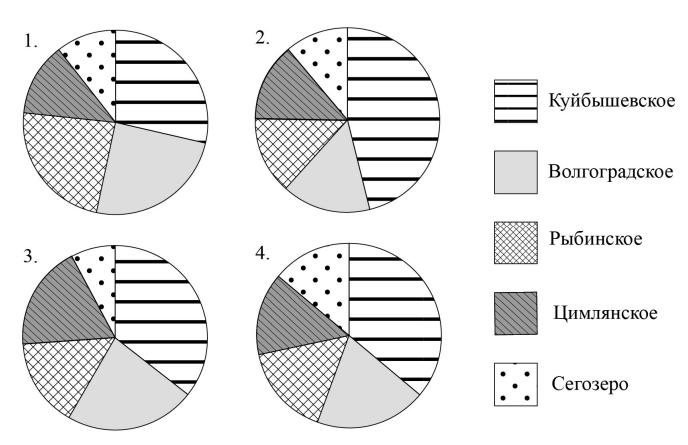
\includegraphics[width=0.54\linewidth]{assets/figure-075.jpg}
\end{center}
\subtask{а)}{Определите, под каким номером приведена верная диаграмма.}
\subtask{б)}{Определите примерный объём Волгоградского водохранилища (в км3).}

\taskspace

\newpage\thispagestyle{fancy}

\item Диаграмма отражает распределение количества посетителей выставки по дням в течение первых 6 дней после её открытия.
\begin{center}
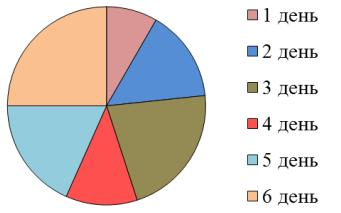
\includegraphics[width=0.54\linewidth]{assets/figure-076.jpg}
\end{center}
\par\medskip\textbf{а)}\enspace Отметьте все утверждения, которые верны, если за эти 6 дней на выставке побывало 12 000 посетителей.
\begin{enumerate}[label=\arabic*),leftmargin=8mm,itemsep=0.25em,topsep=0.35em]
\item В шестой день работы выставки посетителей было больше, чем за первые два дня.
\item За первые 6 дней работы выставки наименьшее количество посетителей было в четвёртый день.
\item В третий день работы выставки на ней побывало от 2000 до 3000 посетителей.
\item За пятый и шестой дни в сумме на выставке побывало от 3000 до 4000 посетителей.
\end{enumerate}
\vspace{0.22cm}
\subtask{б)}{Оцените примерный размах количества посетителей за первые 6 дней работы выставки.}

\taskspace

\newpage\thispagestyle{fancy}

\item Диаграмма отражает распределение количества посетителей выставки по дням в течение первых 6 дней после её открытия.
\begin{center}
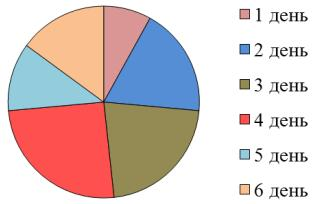
\includegraphics[width=0.54\linewidth]{assets/figure-079.jpg}
\end{center}
\par\medskip\textbf{а)}\enspace Отметьте все утверждения, которые верны, если за эти 6 дней на выставке побывало 8 700 посетителей.
\begin{enumerate}[label=\arabic*),leftmargin=8mm,itemsep=0.25em,topsep=0.35em]
\item В четвёртый день работы выставки посетителей было больше, чем в сумме за первый и шестой дни.
\item За первые 6 дней работы выставки наибольшее количество посетителей было в третий день.
\item За пятый и шестой дни работы выставки на ней побывало от 1500 до 2000 посетителей.
\item С четвёртого по шестой дни на выставке побывало более 4300 посетителей.
\end{enumerate}
\vspace{0.22cm}
\subtask{б)}{Оцените примерный размах количества посетителей за первые 6 дней работы выставки.}

\taskspace

\newpage\thispagestyle{fancy}

\item Диаграмма отражает распределение количества посетителей выставки по дням в течение первых 6 дней после её открытия.
\begin{center}
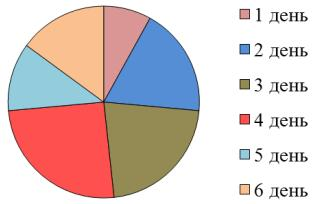
\includegraphics[width=0.54\linewidth]{assets/figure-080.jpg}
\end{center}
\par\medskip\textbf{а)}\enspace Отметьте все утверждения, которые верны, если за эти 6 дней на выставке побывало 5 400 посетителей.
\begin{enumerate}[label=\arabic*),leftmargin=8mm,itemsep=0.25em,topsep=0.35em]
\item За первые 6 дней работы выставки наименьшее количество посетителей было в первый день.
\item За четвёртый и пятый дни на выставке побывало от 2000 до 2700 посетителей.
\item За второй и третий дни работы выставки на ней побывало от 1400 до 2000 посетителей.
\item В первые три дня работы выставки посетителей было меньше, чем в сумме за пятый и шестой дни.
\end{enumerate}
\vspace{0.22cm}
\subtask{б)}{Оцените примерный размах количества посетителей за первые 6 дней работы выставки.}

\taskspace

\newpage\thispagestyle{fancy}

\item В торговом комплексе работает кинотеатр, включающий шесть небольших залов. На диаграмме показано количество мест в каждом из залов.
\begin{center}
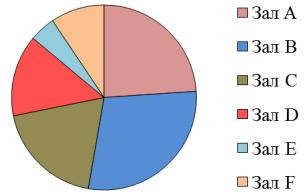
\includegraphics[width=0.54\linewidth]{assets/figure-081.jpg}
\end{center}
\par\medskip\textbf{а)}\enspace Отметьте все утверждения, которые верны, если всего в кинотеатре 330 мест.
\begin{enumerate}[label=\arabic*),leftmargin=8mm,itemsep=0.25em,topsep=0.35em]
\item В зале А больше 85 мест.
\item В зале в от 80 до 110 мест.
\item В кинотеатре есть зал, в котором меньше 40 мест.
\item В зале г мест больше, чем в зале С.
\end{enumerate}
\vspace{0.22cm}
\subtask{б)}{Оцените примерный размах количества мест в указанных залах кинотеатра.}

\taskspace

\newpage\thispagestyle{fancy}

\item B торговом комплексе расположен кинотеатр с шестью небольшими залами. На диаграмме показано количество мест в каждом из залов.
\begin{center}
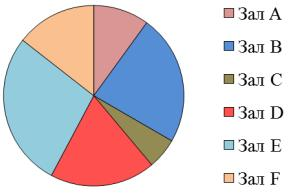
\includegraphics[width=0.54\linewidth]{assets/figure-084.jpg}
\end{center}
\par\medskip\textbf{а)}\enspace Отметьте все утверждения, которые верны, если всего в кинотеатре 360 мест.
\begin{enumerate}[label=\arabic*),leftmargin=8mm,itemsep=0.25em,topsep=0.35em]
\item В зале в меньше 95 мест.
\item В зале о мест меньше, чем в зале А.
\item В зале г от 40 до 60 мест.
\item В кинотеатре есть зал, в котором больше 135 мест.
\end{enumerate}
\vspace{0.22cm}
\subtask{б)}{Оцените примерный размах количества мест в указанных залах кинотеатра.}

\taskspace

\newpage\thispagestyle{fancy}

\item Диаграмма отражает распределение количества посетителей выставки по дням в течение первых 6 дней после её открытия.
\begin{center}
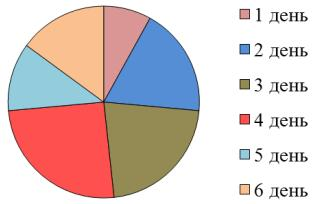
\includegraphics[width=0.54\linewidth]{assets/figure-085.jpg}
\end{center}
\par\medskip\textbf{а)}\enspace Отметьте все утверждения, которые верны, если за эти 6 дней на выставке побывало 10 400 посетителей.
\begin{enumerate}[label=\arabic*),leftmargin=8mm,itemsep=0.25em,topsep=0.35em]
\item За первые 6 дней работы выставки наибольшее количество посетителей было в четвёртый день.
\item За третий и четвёртый дни работы выставки на ней побывало от 4200 до 5100 посетителей.
\item В шестой день работы выставки посетителей было больше, чем во второй день.
\item В первые два дня на выставке побывало от 2600 до 3000 посетителей.
\end{enumerate}
\vspace{0.22cm}
\subtask{б)}{Оцените примерный размах количества посетителей за первые 6 дней работы выставки.}

\taskspace

\newpage\thispagestyle{fancy}

\item B торговом комплексе расположен кинотеатр с шестью небольшими залами. На диаграмме показано количество мест в каждом из залов.
\begin{center}
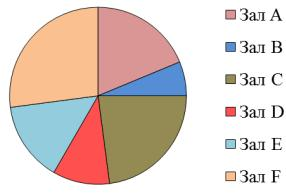
\includegraphics[width=0.54\linewidth]{assets/figure-086.jpg}
\end{center}
\par\medskip\textbf{а)}\enspace Отметьте все утверждения, которые верны, если всего в кинотеатре 240 мест.
\begin{enumerate}[label=\arabic*),leftmargin=8mm,itemsep=0.25em,topsep=0.35em]
\item В зале с от 60 до 90 мест.
\item В зале в меньше 30 мест.
\item В зале D мест больше, чем в зале А.
\item В кинотеатре есть зал, в котором больше 60 мест.
\end{enumerate}
\vspace{0.22cm}
\subtask{б)}{Оцените примерный размах количества мест в указанных залах кинотеатра.}

\taskspace

\newpage\thispagestyle{fancy}

\item На диаграмме показано количество посетителей выставки (по дням) за первые 6 дней после её открытия.
\begin{center}
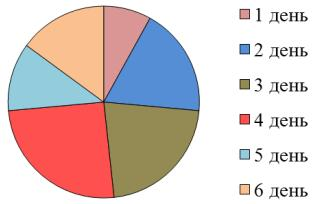
\includegraphics[width=0.54\linewidth]{assets/figure-087.jpg}
\end{center}
\par\medskip\textbf{а)}\enspace Отметьте все утверждения, которые верны, если за эти 6 дней на выставке побывало 12 000 посетителей.
\begin{enumerate}[label=\arabic*),leftmargin=8mm,itemsep=0.25em,topsep=0.35em]
\item В шестой день работы выставки посетителей было больше, чем за первые два дня.
\item За первые 6 дней работы выставки наименьшее количество посетителей было в четвёртый день.
\item В третий день работы выставки на ней побывало от 2000 до 3000 посетителей.
\item За пятый и шестой дни в сумме на выставке побывало от 3000 до 4000 посетителей.
\end{enumerate}
\vspace{0.22cm}
\subtask{б)}{Оцените примерный размах количества посетителей за первые 6 дней работы выставки.}

\taskspace

\newpage\thispagestyle{fancy}

\item Сплавляются два вещества, состоящие из серы, железа, водорода и меди. Массовые доли серы (S), железа (Fe), водорода (Н) и меди (Cu) в каждом веществе приведены на диаграммах.
\begin{center}
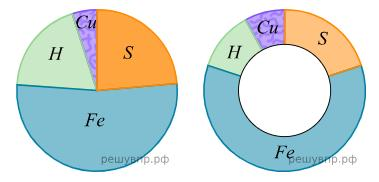
\includegraphics[width=0.78\linewidth]{assets/figure-090.jpg}
\end{center}
\begin{center}
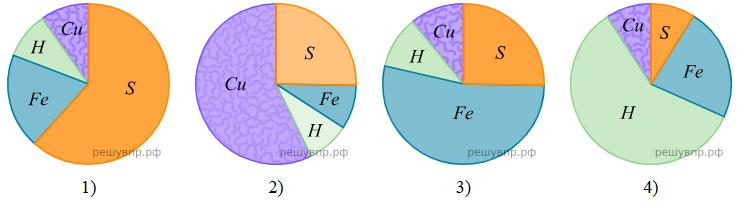
\includegraphics[width=0.78\linewidth]{assets/figure-091.jpg}
\end{center}
\subtask{а)}{Установите, какая из диаграмм правильно отражает соотношение элементов в сплаве.}
\subtask{б)}{Установите, на какой из диаграмм приведен состав вещества, более половины состава которого составляет медь.}

\taskspace

\newpage\thispagestyle{fancy}

\item Численность населения измеряют в миллионах человек (млн чел.). В таблице указаны некоторые описательные характеристики численности населения пяти крупнейших субъектов Российской Федерации: г. Москвы, Московской области, Краснодарского края, г. Санкт-Петербурга и Свердловской области на начало 2022 г. Далее приведены четыре диаграммы, показывающие долю численности населения каждого субъекта в суммарной численности населения этих субъектов. Только одна из диаграмм верная.
\begin{center}
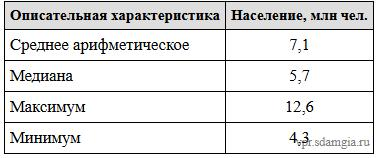
\includegraphics[width=0.78\linewidth]{assets/figure-092.jpg}
\end{center}
\begin{center}
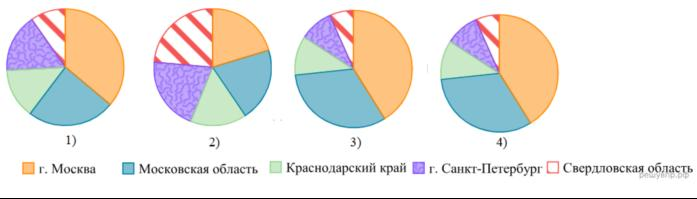
\includegraphics[width=0.78\linewidth]{assets/figure-093.jpg}
\end{center}
\subtask{а)}{Определите, под каким номером приведена верная диаграмма.}
\subtask{б)}{Определите примерную численность населения Краснодарского края (млн чел).}

\taskspace

\newpage\thispagestyle{fancy}

\item Площадь горных систем измеряют в тысячах квадратных километров (тыс. км2). В таблице указаны некоторые описательные характеристики площадей пяти высочайших горных систем мира: Гималаи, Каракорума, Куньлуня, Иранского нагорья и Памира. Далее приведены четыре диаграммы, показывающие долю каждой горной системы в суммарной площади этих горных систем. Только одна из диаграмм верная.
\begin{center}
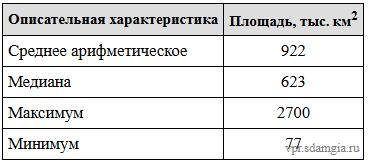
\includegraphics[width=0.78\linewidth]{assets/figure-097.jpg}
\end{center}
\begin{center}
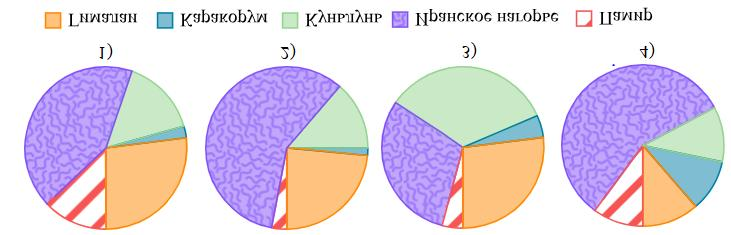
\includegraphics[width=0.78\linewidth]{assets/figure-098.jpg}
\end{center}
\subtask{а)}{Определите, под каким номером приведена верная диаграмма.}
\subtask{б)}{Определите примерную площадь горной системы Каракорум (в тыс. км2).}

\taskspace

\newpage\thispagestyle{fancy}

\item Площадь горных систем измеряют в тысячах квадратных километров (тыс. кв. км). В таблице указаны некоторые описательные характеристики площадей пяти высочайших горных систем мира: Гималаи, Каракорум, Куньлунь, Иранское нагорье и Памир. Далее приведены четыре диаграммы, показывающие долю каждой горной системы в их суммарной площади. Только одна из диаграмм верная.
\begin{center}
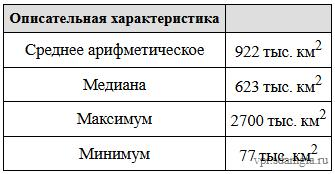
\includegraphics[width=0.78\linewidth]{assets/figure-099.jpg}
\end{center}
\begin{center}
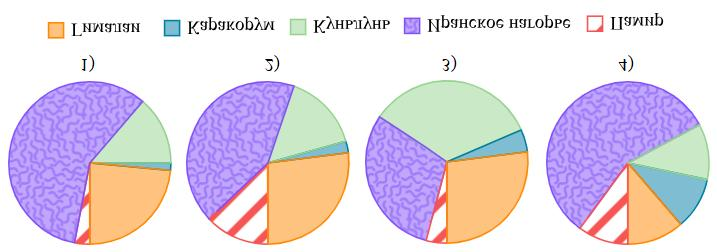
\includegraphics[width=0.78\linewidth]{assets/figure-100.jpg}
\end{center}
\subtask{а)}{Определите, под каким номером приведена верная диаграмма.}
\subtask{б)}{Вычислите площадь горной системы Куньлунь (в тыс. км2).}

\taskspace

\newpage\thispagestyle{fancy}

\item В таблице собраны данные о численности населения пяти крупнейших субъектов Российской Федерации: г. Москва, Московская область, Краснодарский край, г. Санкт-Петербург и Свердловская область на начало 2022 г. Далее приведены четыре диаграммы, показывающие долю численности населения каждого субъекта в их общей численности. Только одна из диаграмм верная.
\begin{center}
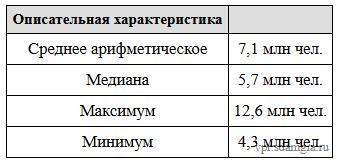
\includegraphics[width=0.78\linewidth]{assets/figure-103.jpg}
\end{center}
\begin{center}
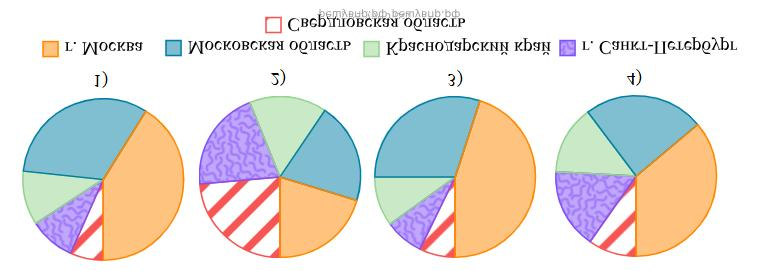
\includegraphics[width=0.78\linewidth]{assets/figure-104.jpg}
\end{center}
\subtask{а)}{Далее приведены четыре диаграммы, показывающие долю численности населения каждого субъекта в их общей численности. Только одна из диаграмм верная.}
\subtask{б)}{Определите численность населения Свердловской области (млн чел.).}

\taskspace

\newpage\thispagestyle{fancy}

\item Урожайность сельскохозяйственных культур измеряют в центнерах с одного гектара убранной площади (ц/га). В таблице указаны некоторые описательные характеристики урожайности нескольких сельскохозяйственных культур России: подсолнечника, зерновых и зернобобовых культур, овощей, сахарной свёклы и картофеля. Далее приведены четыре диаграммы, показывающие урожайность каждой культуры. Только одна из диаграмм верная.
\begin{center}
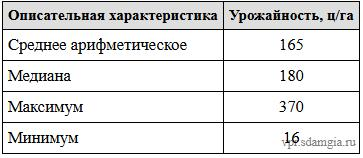
\includegraphics[width=0.78\linewidth]{assets/figure-105.jpg}
\end{center}
\begin{center}
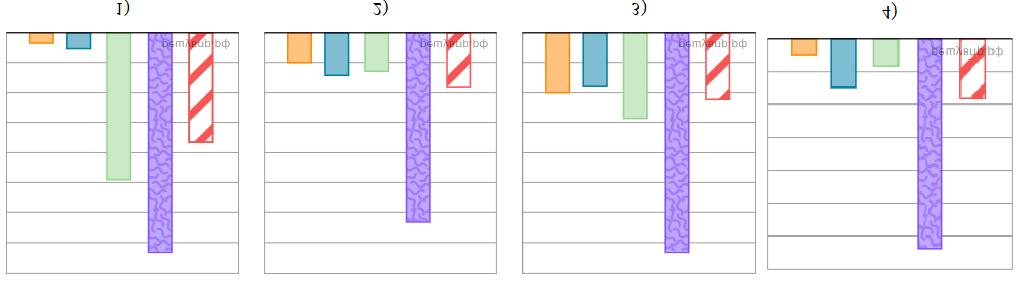
\includegraphics[width=0.78\linewidth]{assets/figure-106.jpg}
\end{center}
\subtask{а)}{Определите, под каким номером приведена верная диаграмма.}
\subtask{б)}{Определите урожайность сахарной свеклы (в ц/га).}

\taskspace

\end{enumerate}

\newpage

\section*{Блок VII. Задание МЦКО 7}

\blocknote{Вероятность и статистика: графы.}

\begin{enumerate}[resume]

\Needspace{6\baselineskip}
\item В данном графе семь вершин степени 4 и ещё шесть вершин степени 3. Других вершин в этом графе нет. Определите число рёбер этого графа.

\taskspace

\Needspace{6\baselineskip}
\item Половина вершин данного графа имеет степень 5, а половина --- степень 3. Каково число вершин этого графа, если в нём 48 ребер?

\taskspace

\Needspace{6\baselineskip}
\item Половина вершин данного графа имеет степень 3, а половина - степень 4. Каково число вершин этого графа, если в нём 56 ребер?

\taskspace

\Needspace{6\baselineskip}
\item Половина вершин данного графа имеет степень 5, а половина - степень 4. Каково число вершин этого графа, если в нём 45 ребер?

\taskspace

\Needspace{6\baselineskip}
\item Половина вершин данного графа имеет степень 4, а половина - степень 6. Каково число вершин этого графа, если в нём 30 рёбер?

\taskspace

\Needspace{6\baselineskip}
\item Половина вершин данного графа имеет степень 3, а половина - степень 4. Каково число вершин этого графа, если в нём 42 ребра?

\taskspace

\Needspace{6\baselineskip}
\item Половина вершин данного графа имеет степень 5, а половина - степень 4. Каково число вершин этого графа, если в нём 36 рёбер?

\taskspace

\Needspace{6\baselineskip}
\item Половина вершин данного графа имеет степень 4, а половина - степень 6. Каково число вершин этого графа, если в нём 40 рёбер?

\taskspace

\Needspace{6\baselineskip}
\item Половина вершин данного графа имеет степень 5, а половина - степень 3. Каково число вершин этого графа, если в нём 40 рёбер?

\taskspace

\Needspace{6\baselineskip}
\item Рассматривается граф, в котором 5 вершин и 7 рёбер. Три вершины имеют степень 2, четвёртая вершина --- степень 3. Какова степень пятой вершины?

\taskspace

\Needspace{6\baselineskip}
\item В графе 10 вершин: две вершины степени 9 и ещё восемь вершин степени 6. Определите число рёбер этого графа.

\taskspace

\Needspace{6\baselineskip}
\item Рассматривается граф, в котором 9 вершин, степени которых равны 2, 3, 3, 5, 5, 7, 7, 9, 9. Определите число рёбер этого графа.

\taskspace

\Needspace{6\baselineskip}
\item Рассматривается граф, в котором 8 вершин, степени которых равны 3, 3, 4, 4, 5, 5, 6, 6. Определите число рёбер этого графа.

\taskspace

\Needspace{6\baselineskip}
\item Рассматривается граф, в котором 14 рёбер. Каждая вершина графа имеет степень 2 или степень 5, причём вершин степени 2 и степени 5 поровну. Других вершин в этом графе нет. Сколько всего вершин содержит граф?

\taskspace

\Needspace{6\baselineskip}
\item Рассматривается граф, в котором 20 рёбер. Каждая вершина графа имеет степень 2 или степень 3, причём вершин степени 2 столько же, сколько вершин степени 3. Сколько всего вершин содержит граф?

\taskspace

\Needspace{6\baselineskip}
\item Рассматривается граф, в котором 33 ребра. Каждая вершина графа имеет степень 4 или степень 7, причём вершин степени 4 столько же, сколько вершин степени 7. Сколько всего вершин содержит граф?

\taskspace

\Needspace{6\baselineskip}
\item Рассматривается граф, в котором 11 рёбер. Пять вершин имеют степень 2, а остальные вершины --- степень 3. Других вершин в этом графе нет. Сколько вершин степени 3 содержит граф?

\taskspace

\Needspace{6\baselineskip}
\item Рассматривается граф, в котором 11 рёбер. Пять вершин имеют степень 2, а остальные вершины --- степень 3. Других вершин в этом графе нет. Сколько вершин степени 3 содержит граф?

\taskspace

\Needspace{6\baselineskip}
\item В графе 12 рёбер, а каждая вершина имеет индекс 3. Других вершин в этом графе нет. Определите число вершин данного графа.

\taskspace

\Needspace{6\baselineskip}
\item В графе 45 рёбер, а каждая вершина имеет индекс 9. Других вершин в этом графе нет. Определите число вершин данного графа.

\taskspace

\Needspace{6\baselineskip}
\item В данном графе 7 вершин степени 4 и еще 6 вершин степени 3. Других вершин в этом графе нет. Определите число рёбер этого графа.

\taskspace

\Needspace{6\baselineskip}
\item В графе 5 вершин, каждая из которых имеет индекс 4. Других вершин в этом графе нет. Определите число рёбер данного графа.

\taskspace

\Needspace{6\baselineskip}
\item В графе 4 вершины, каждая из которых имеет индекс 3. Других вершин в этом графе нет. Определите число рёбер данного графа.

\taskspace

\Needspace{6\baselineskip}
\item В графе 8 вершин степени 5 и ещё 5 вершин степени 4. Других вершин в этом графе нет. Определите число рёбер данного графа.

\taskspace

\Needspace{6\baselineskip}
\item В данном графе девять вершин степени 3 и ещё шесть вершин степени 5. Других вершин в этом графе нет. Определите число рёбер этого графа.

\taskspace

\Needspace{6\baselineskip}
\item В данном графе десять вершин степени 4 и ещё восемь вершин степени 3. Других вершин в этом графе нет. Определите число рёбер этого графа.

\taskspace

\Needspace{6\baselineskip}
\item В данном графе шесть вершин степени 5 и ещё десять вершин степени 3. Других вершин в этом графе нет. Определите число рёбер этого графа.

\taskspace

\Needspace{6\baselineskip}
\item В данном графе пять вершин степени 6 и ещё девять вершин степени 4. Других вершин в этом графе нет. Определите число рёбер этого графа.

\taskspace

\Needspace{6\baselineskip}
\item В данном графе двенадцать вершин степени 3 и ещё четыре вершины степени 5. Других вершин в этом графе нет. Определите число рёбер этого графа.

\taskspace

\Needspace{6\baselineskip}
\item В данном графе восемь вершин степени 3 и ещё шесть вершин степени 4. Других вершин в этом графе нет. Определите число рёбер этого графа.

\taskspace

\end{enumerate}

\newpage

\section*{Блок VIII. Задание МЦКО 8}

\blocknote{Статистические характеристики.}

\begin{enumerate}[resume]

\Needspace{6\baselineskip}
\item В институте используется десятибалльная система оценки знаний студентов. Средняя оценка вычисляется как среднее арифметическое. Преподаватель дал одну и ту же контрольную работу в двух группах. Результаты представлены в таблице.
\begin{center}
\renewcommand{\arraystretch}{1.22}
\begin{tabular}{@{}lcc@{}}\textbf{Группа} & \textbf{1} & \textbf{2} \\
Число студентов & 20 & 30 \\
Средняя оценка & 8,2 & 7,8\end{tabular}
\end{center}
\subtask{а)}{Вычислите среднюю оценку всех студентов за эту работу.}
\subtask{б)}{Несколько студентов переписали работу, и каждый получил на 1 балл больше, чем при первой попытке. В результате средняя оценка всех студентов стала равной 8. Сколько студентов переписало работу?}

\taskspace

\Needspace{6\baselineskip}
\item Таблица содержит сведения о среднем расходе топлива в литрах на сто километров пробега автомобиля в тёплое и холодное время года, а также о пробеге автомобиля в эти периоды.
\begin{center}
\renewcommand{\arraystretch}{1.22}
\begin{tabular}{@{}lcc@{}}\textbf{Время года} & \textbf{Тёплое} & \textbf{Холодное} \\
Пробег, тыс. км & 11 & 9 \\
Расход топлива, л/100 км & 8 & 10\end{tabular}
\end{center}
\subtask{а)}{Определите средний расход топлива в литрах на сто километров пробега этого автомобиля за весь год.}
\subtask{б)}{Если бы этот автомобиль оборудовали кондиционером, то расход топлива в тёплое время года увеличился бы на 1 л на 100 км. На сколько увеличился бы средний расход топлива за весь год? Укажите ответ в литрах на сто километров пробега.}

\taskspace

\Needspace{6\baselineskip}
\item Таблица содержит сведения о среднем расходе топлива в литрах на сто километров пробега автомобиля в тёплое и холодное время года, а также о пробеге автомобиля в эти периоды.
\begin{center}
\renewcommand{\arraystretch}{1.22}
\begin{tabular}{@{}lcc@{}}\textbf{Время года} & \textbf{Тёплое} & \textbf{Холодное} \\
Пробег, тыс. км & 14 & 6 \\
Расход топлива, л/100 км & 10 & 12\end{tabular}
\end{center}
\subtask{а)}{Определите средний расход топлива в литрах на сто километров пробега этого автомобиля за весь год.}
\subtask{б)}{Если бы этот автомобиль оборудовали кондиционером, то расход топлива в тёплое время года увеличился бы на 1 л на 100 км. На сколько увеличился бы средний расход топлива за весь год? Укажите ответ в литрах на сто километров пробега.}

\taskspace

\Needspace{6\baselineskip}
\item Таблица содержит сведения о среднем расходе топлива в литрах на сто километров пробега автомобиля в тёплое и холодное время года, а также о пробеге автомобиля в эти периоды.
\begin{center}
\renewcommand{\arraystretch}{1.22}
\begin{tabular}{@{}lcc@{}}\textbf{Время года} & \textbf{Тёплое} & \textbf{Холодное} \\
Пробег, тыс. км & 12 & 8 \\
Расход топлива, л/100 км & 9 & 12\end{tabular}
\end{center}
\subtask{а)}{Определите средний расход топлива в литрах на сто километров пробега этого автомобиля за весь год.}
\subtask{б)}{Если бы этот автомобиль оборудовали кондиционером, то расход топлива в тёплое время года увеличился бы на 1 л на 100 км. На сколько увеличился бы средний расход топлива за весь год? Укажите ответ в литрах на сто километров пробега.}

\taskspace

\Needspace{6\baselineskip}
\item Таблица содержит сведения о среднем расходе топлива в литрах на сто километров пробега автомобиля в тёплое и холодное время года, а также о пробеге автомобиля в эти периоды.
\begin{center}
\renewcommand{\arraystretch}{1.22}
\begin{tabular}{@{}lcc@{}}\textbf{Время года} & \textbf{Тёплое} & \textbf{Холодное} \\
Пробег, тыс. км & 18 & 2 \\
Расход топлива, л/100 км & 10 & 13\end{tabular}
\end{center}
\subtask{а)}{Определите средний расход топлива в литрах на сто километров пробега этого автомобиля за весь год.}
\subtask{б)}{Если бы этот автомобиль оборудовали кондиционером, то расход топлива в тёплое время года увеличился бы на 1 л на 100 км. На сколько увеличился бы средний расход топлива за весь год? Укажите ответ в литрах на сто километров пробега.}

\taskspace

\Needspace{6\baselineskip}
\item Таблица содержит сведения о среднем расходе топлива в литрах на сто километров пробега автомобиля в тёплое и холодное время года, а также о пробеге автомобиля в эти периоды.
\begin{center}
\renewcommand{\arraystretch}{1.22}
\begin{tabular}{@{}lcc@{}}\textbf{Время года} & \textbf{Тёплое} & \textbf{Холодное} \\
Пробег, тыс. км & 17 & 3 \\
Расход топлива, л/100 км & 8 & 10\end{tabular}
\end{center}
\subtask{а)}{Определите средний расход топлива в литрах на сто километров пробега этого автомобиля за весь год.}
\subtask{б)}{Если бы этот автомобиль оборудовали кондиционером, то расход топлива в тёплое время года увеличился бы на 1 л на 100 км. На сколько увеличился бы средний расход топлива за весь год? Укажите ответ в литрах на сто километров пробега.}

\taskspace

\Needspace{6\baselineskip}
\item Таблица содержит сведения о среднем расходе топлива в литрах на сто километров пробега автомобиля в тёплое и холодное время года, а также о пробеге автомобиля в эти периоды.
\begin{center}
\renewcommand{\arraystretch}{1.22}
\begin{tabular}{@{}lcc@{}}\textbf{Время года} & \textbf{Тёплое} & \textbf{Холодное} \\
Пробег, тыс. км & 15 & 5 \\
Расход топлива, л/100 км & 9 & 11\end{tabular}
\end{center}
\subtask{а)}{Определите средний расход топлива в литрах на сто километров пробега этого автомобиля за весь год.}
\subtask{б)}{Если бы этот автомобиль оборудовали кондиционером, то расход топлива в тёплое время года увеличился бы на 1 л на 100 км. На сколько увеличился бы средний расход топлива за весь год? Укажите ответ в литрах на сто километров пробега.}

\taskspace

\Needspace{6\baselineskip}
\item Таблица содержит сведения о среднем расходе топлива в литрах на сто километров пробега автомобиля в тёплое и холодное время года, а также о пробеге автомобиля в эти периоды.
\begin{center}
\renewcommand{\arraystretch}{1.22}
\begin{tabular}{@{}lcc@{}}\textbf{Время года} & \textbf{Тёплое} & \textbf{Холодное} \\
Пробег, тыс. км & 13 & 7 \\
Расход топлива, л/100 км & 9 & 11\end{tabular}
\end{center}
\subtask{а)}{Определите средний расход топлива в литрах на сто километров пробега этого автомобиля за весь год.}
\subtask{б)}{Если бы этот автомобиль оборудовали кондиционером, то расход топлива в тёплое время года увеличился бы на 1 л на 100 км. На сколько увеличился бы средний расход топлива за весь год? Укажите ответ в литрах на сто километров пробега.}

\taskspace

\Needspace{6\baselineskip}
\item Таблица содержит сведения о среднем расходе топлива в литрах на сто километров пробега автомобиля в тёплое и холодное время года, а также о пробеге автомобиля в эти периоды.
\begin{center}
\renewcommand{\arraystretch}{1.22}
\begin{tabular}{@{}lcc@{}}\textbf{Время года} & \textbf{Тёплое} & \textbf{Холодное} \\
Пробег, тыс. км & 16 & 4 \\
Расход топлива, л/100 км & 10 & 12\end{tabular}
\end{center}
\subtask{а)}{Определите средний расход топлива в литрах на сто километров пробега этого автомобиля за весь год.}
\subtask{б)}{Если бы этот автомобиль оборудовали кондиционером, то расход топлива в тёплое время года увеличился бы на 1 л на 100 км. На сколько увеличился бы средний расход топлива за весь год? Укажите ответ в литрах на сто километров пробега.}

\taskspace

\Needspace{6\baselineskip}
\item Для компота из сухофруктов приобрели яблоки, изюм и курагу. Их цены и количество указаны в таблице.
\begin{center}
\renewcommand{\arraystretch}{1.22}
\begin{tabular}{@{}lccc@{}}\textbf{Ингредиенты} & \textbf{Яблоки} & \textbf{Изюм} & \textbf{Курага} \\
Цена, руб./кг & 15 & 215 & 635 \\
Количество, кг & 3 & 1,2 & 1,8\end{tabular}
\end{center}
\subtask{а)}{Вычислите среднюю стоимость 1 кг полученной смеси сухофруктов. Укажите ответ в рублях.}
\subtask{б)}{После того как в дополнение к указанным ингредиентам купили чернослив по цене 651 рубль за 1 кг, стоимость 1 кг смеси сухофруктов стала равна 376 рублей. Определите массу купленного чернослива в килограммах.}

\taskspace

\Needspace{6\baselineskip}
\item Для компота из сухофруктов приобрели яблоки, изюм и курагу. Их цены и количество указаны в таблице.
\begin{center}
\renewcommand{\arraystretch}{1.22}
\begin{tabular}{@{}lccc@{}}\textbf{Ингредиенты} & \textbf{Яблоки} & \textbf{Изюм} & \textbf{Курага} \\
Цена, руб./кг & 170 & 210 & 590 \\
Количество, кг & 3 & 1 & 1\end{tabular}
\end{center}
\subtask{а)}{Вычислите среднюю стоимость 1 кг полученной смеси сухофруктов. Укажите ответ в рублях.}
\subtask{б)}{После того как в дополнение к указанным ингредиентам купили чернослив по цене 900 рублей за 1 кг, стоимость 1 кг смеси сухофруктов стала равна 350 рублей. Определите массу купленного чернослива в килограммах.}

\taskspace

\Needspace{6\baselineskip}
\item Для компота из сухофруктов приобрели яблоки, изюм и курагу. Их цены и количество указаны в таблице.
\begin{center}
\renewcommand{\arraystretch}{1.22}
\begin{tabular}{@{}lccc@{}}\textbf{Ингредиенты} & \textbf{Яблоки} & \textbf{Изюм} & \textbf{Курага} \\
Цена, руб./кг & 180 & 230 & 610 \\
Количество, кг & 1 & 0,7 & 0,3\end{tabular}
\end{center}
\subtask{а)}{Вычислите среднюю стоимость 1 кг полученной смеси сухофруктов. Укажите ответ в рублях.}
\subtask{б)}{После того как в дополнение к указанным ингредиентам купили чернослив по цене 842 рубля за 1 кг, стоимость 1 кг смеси сухофруктов стала равна 382 рубля. Определите массу купленного чернослива в килограммах.}

\taskspace

\Needspace{6\baselineskip}
\item Для компота из сухофруктов приобрели яблоки, изюм и курагу. Их цены и количество указаны в таблице.
\begin{center}
\renewcommand{\arraystretch}{1.22}
\begin{tabular}{@{}lccc@{}}\textbf{Ингредиенты} & \textbf{Яблоки} & \textbf{Изюм} & \textbf{Курага} \\
Цена, руб./кг & 180 & 225 & 600 \\
Количество, кг & 3,2 & 0,8 & 2\end{tabular}
\end{center}
\subtask{а)}{Вычислите среднюю стоимость 1 кг полученной смеси сухофруктов. Укажите ответ в рублях.}
\subtask{б)}{После того как в дополнение к указанным ингредиентам купили чернослив по цене 865 рублей за 1 кг, стоимость 1 кг смеси сухофруктов стала равна 375 рублей. Определите массу купленного чернослива в килограммах.}

\taskspace

\Needspace{6\baselineskip}
\item Для компота из сухофруктов приобрели яблоки, изюм и курагу. Их цены и количество указаны в таблице.
\begin{center}
\renewcommand{\arraystretch}{1.22}
\begin{tabular}{@{}lccc@{}}\textbf{Ингредиенты} & \textbf{Яблоки} & \textbf{Изюм} & \textbf{Курага} \\
Цена, руб./кг & 160 & 250 & 650 \\
Количество, кг & 2 & 1,3 & 0,7\end{tabular}
\end{center}
\subtask{а)}{Вычислите среднюю стоимость 1 кг полученной смеси сухофруктов. Укажите ответ в рублях.}
\subtask{б)}{После того как в дополнение к указанным ингредиентам купили чернослив по цене 946 рублей за 1 кг, стоимость 1 кг смеси сухофруктов стала равна 506 рублей. Определите массу купленного чернослива в килограммах.}

\taskspace

\Needspace{6\baselineskip}
\item В таблице приведены сведения о двух линиях московского метрополитена на 2022 г.: количество станций, протяжённость линии и время поездки между конечными станциями.
\begin{center}
\renewcommand{\arraystretch}{1.22}
\begin{tabularx}{0.96\linewidth}{@{}Xccc@{}}\textbf{Название линии} & \textbf{Станций} & \textbf{Длина, км} & \textbf{Время, мин} \\
Серпуховско-Тимирязевская & 25 & 44,2 & 58 \\
Замоскворецкая & 24 & 42,8 & 62\end{tabularx}
\end{center}
\subtask{а)}{Определите среднюю продолжительность поездки между двумя соседними станциями Замоскворецкой линии. Ответ выразите в минутах. Результат округлите до десятых.}
\subtask{б)}{Определите среднее расстояние между соседними станциями Серпуховско-Тимирязевской линии. Укажите ответ в километрах с округлением до сотых.}

\taskspace

\end{enumerate}


\vfill
{\small\color{soft}Работа завершена. Пропуски помогут определить темы для дальнейшего повторения.}
\end{document}
